%% Modified documentstyle to documentclass -- compatibility with LaTex2e
%% N. Mancell (98/03/01).

%%  ucalgthes_root.tex        (NM 98/03/01)
%   Modified   92-09-18      Add references to dissertation        D. Teale
%                            Add approval page to toc
%                            Add ref to Title Degree on approval page
%   Modified  2006-09-12     Added geometry package to set up UofC thesis margins
%                            Removed includeprompt option N. Mancell
%
\documentclass{ucalgthes1}   
\usepackage[letterpaper,top=1in, bottom=1.22in, left=1.40in, right=0.850in]{geometry}
\usepackage{fancyhdr}
\fancyhead{}
\fancyfoot{}
\renewcommand{\headrulewidth}{0pt}
\fancyhead[RO,LE]{\thepage}  



%Define other usepackages here
\usepackage[T1]{pbsi}
\usepackage{t1enc,dfadobe}
\usepackage{cite}
\usepackage{framed}
\usepackage{newalg}
\usepackage{subfigure}
\usepackage{graphics}
\usepackage{graphicx}
\usepackage{amsmath}
\usepackage{amssymb}
\usepackage{amsmath}
\usepackage{tocloft}
\usepackage[titles]{tocloft}
\usepackage{trivfloat}
\usepackage{float}
\usepackage{hyperref}
\usepackage[numbered]{algorithm}
\usepackage{algorithmic}

\hypersetup{
    bookmarks=true,         % show bookmarks bar?
    unicode=false,          % non-Latin characters in Acrobat�s bookmarks
    pdftoolbar=true,        % show Acrobat�s toolbar?
    pdfmenubar=true,        % show Acrobat�s menu?
    pdftitle={Level Set Volume Segmentation using Programmable Graphics Hardware},    % title
    pdfauthor={Mike Roberts},     % author
    pdfnewwindow=true,      % links in new window
    pdfborder={0,0,0},
    colorlinks=false,       % false: boxed links; true: colored links
    linkcolor=red,          % color of internal links
    citecolor=green,        % color of links to bibliography
    filecolor=magenta,      % color of file links
    urlcolor=cyan           % color of external links
}


% Alter some LaTeX defaults for better treatment of figures:
% See p.105 of "TeX Unbound" for suggested values.
% See pp. 199-200 of Lamport's "LaTeX" book for details.
%   General parameters, for ALL pages:
\renewcommand{\topfraction}{0.9}    % max fraction of floats at top
\renewcommand{\bottomfraction}{0.8} % max fraction of floats at bottom
%   Parameters for TEXT pages (not float pages):
\setcounter{topnumber}{2}
\setcounter{bottomnumber}{2}
\setcounter{totalnumber}{4}     % 2 may work better
\setcounter{dbltopnumber}{2}    % for 2-column pages
\renewcommand{\dbltopfraction}{0.9} % fit big float above 2-col. text
\renewcommand{\textfraction}{0.07}  % allow minimal text w. figs
%   Parameters for FLOAT pages (not text pages):
\renewcommand{\floatpagefraction}{0.7}      % require fuller float pages
    % N.B.: floatpagefraction MUST be less than topfraction !!
\renewcommand{\dblfloatpagefraction}{0.7}   % require fuller float pages

% remember to use [htp] or [htpb] for placement




\floatstyle{boxed}
\trivfloat{Listing}




\renewcommand{\contentsname}{Table of Contents}
\renewcommand{\listfigurename}{List of Figures}

\renewcommand{\cfttoctitlefont}{\Large\hfill}
\renewcommand{\cftaftertoctitle}{\hfill}

\renewcommand{\cftloftitlefont}{\Large\hfill}
\renewcommand{\cftafterloftitle}{\hfill}

\setlength{\cftbeforetoctitleskip}{-0.175in}
\setlength{\cftaftertoctitleskip}{0.3in}
\setlength{\cftbeforeloftitleskip}{-0.145in}
\setlength{\cftafterloftitleskip}{0.335in}



\newcommand{\leftbracket}{\left(}
\newcommand{\rightbracket}{\right)}

\newcommand{\leftcbracket}{\left\{}
\newcommand{\rightcbracket}{\right\}}

\newcommand{\leftvbracket}{\left|}
\newcommand{\rightvbracket}{\right|}

\newcommand{\leftsbracket}{\left[}
\newcommand{\rightsbracket}{\right]}

\newcommand{\boldx}{{\mathbf x}}
\newcommand{\boldn}{{\mathbf n}}
\newcommand{\boldv}{{\mathbf v}}
\newcommand{\boldy}{{\mathbf y}}

\newcommand{\phixt}{ \mathit{\phi} \leftbracket \boldx , t \rightbracket }
\newcommand{\phixtmdt}{ \mathit{\phi} \leftbracket \boldx , t - \Delta t \rightbracket }
\newcommand{\phixtmtdt}{ \mathit{\phi} \leftbracket \boldx , t - 2 \Delta t \rightbracket }

\newcommand{\conditionone}{ { \varsigma }_{1} \leftbracket \boldx , t \rightbracket }
\newcommand{\conditiontwo}{ { \varsigma }_{2} \leftbracket \boldx , t \rightbracket }

\newcommand{\ix}{I \leftbracket \boldx \rightbracket}

\newcommand{\nx}{ \eta \leftbracket \boldx \rightbracket }
\newcommand{\nv}{ \eta \leftbracket \boldv \rightbracket }
\newcommand{\nn}{ \eta \leftbracket \boldn \rightbracket }

\newcommand{\curvatureterm}{ \nabla \cdot \frac{\nabla \phixtmdt }{ \leftvbracket \nabla \phixtmdt \rightvbracket } }

\newcommand{\phiread}{ \phi^{read} }
\newcommand{\phiwrite}{ \phi^{write} }

\newcommand{\domainphi}{ \mbox{Domain} \leftbracket \phi \rightbracket }
\newcommand{\domainphiread}{ \mbox{Domain} \leftbracket \phiread \rightbracket }
\newcommand{\domainphiwrite}{ \mbox{Domain} \leftbracket \phiwrite \rightbracket }
\newcommand{\domainu}{ \mbox{Domain} \leftbracket U \rightbracket }

\newcommand{\qed}{\hfill \ensuremath{\Box}}

\newtheorem{cla}{Claim}
\newtheorem{lem}{Lemma}
\newtheorem{pro}{Proof}




\title{Level Set Volume Segmentation using Programmable Graphics Hardware}
\author{Mike Roberts}
\thesisyear{2011}
\thesis{thesis}
\newcommand{\thesistitle}{Level Set Volume Segmentation using Programmable Graphics Hardware}
\monthname{April}
\dept{COMPUTER SCIENCE}
\degree{MASTER OF SCIENCE}






\begin{document}

\makethesistitle
\pagenumbering{roman}     % resets page counter to one
\setcounter{page}{1}
\chapter*{UNIVERSITY OF CALGARY \\ FACULTY OF GRADUATE STUDIES}
\thispagestyle{empty}
The undersigned certify that they have read, and recommend
to the Faculty of Graduate Studies for acceptance, a \Thesis\ entitled
``\thesistitle'' submitted by \Author\
in partial fulfillment of the requirements for the degree of \Degree.\\




%
%                 Substitute  List of Examiners
%
\begin{signing}{Department of Academic Computing}



%\newsigncolumn         use this command to start a new column if necessary



\newsigncolumn
\signline
Dr.~Mario Costa Sousa \\
Department of Computer Science \\
\signline
Dr.~Joseph Ross Mitchell \\
Departments of Clinical Neurosciences and Radiology \\
\signline
Dr.~Christian Jacob \\
Department of Computer Science \\
\signline
Dr.~Mayank Goyal \\
Department of Radiology \\
\end{signing}

\newpage
\phantomsection
\altchapter{Abstract}

Identifying distinct regions in images -- a task known as \emph{segmentation} -- is an important task in computer vision and diagnostic medicine. The level set method is a powerful, flexible, and accurate numerical technique for image segmentation under challenging conditions since the segmentation process can depend on image properties (e.g. color or texture) and can enforce geometric constraints (e.g. smoothness) on the segmented regions. However, the flexibility of the level set method has historically resulted in long computation times and therefore limited clinical utility. In this thesis I describe a novel parallel level set segmentation algorithm that dramatically improves computational efficiency without affecting segmentation accuracy.

The level set method for image segmentation~begins with an implicitly represented seed surface embedded within a regular scalar grid. The level set method deforms this surface to envelop a corresponding region-of-interest in the original image by iteratively solving a partial differential equation defined at each grid element. Previous algorithms avoid unnecessary  computations by updating only those
grid elements near the deforming surface.

In this thesis I prove that even computations near the surface can be avoided in regions where the grid has locally converged. I describe a novel parallel algorithm  that leverages this insight and performs $O(n)$ work in $O(\log_2 n)$ steps, in contrast to previous parallel algorithms which perform  $O(n)$ work in $O(n)$ steps. I apply my algorithm to 3D medical images and I demonstrate significant peformance advantages over previous algorithms. In typical clinical scenarios, my algorithm reduces the total number of processed grid elements by $16 \times$ and is $14 \times$ faster than previous parallel algorithms with equal accuracy in all experiments. My algorithm runs entirely on commodity graphics processing units without requiring any additional data processing on the CPU, thereby enabling interactive 3D visualization and real-time control of the evolving segmentation.




 
\newpage
\phantomsection
\thispagestyle{plain}

\vspace*{\fill}
\begingroup
\centering

\begin{LARGE}

\textbsi{To Chelsea}

\textbsi{(the blonde science nerd from heaven)}

\end{LARGE}

\endgroup
\vspace*{\fill}

\newpage
\phantomsection
\altchapter{Acknowledgments}

\thispagestyle{plain}

It is a pleasure to thank the many people that made this thesis possible.

I want to thank my advisors, Dr. Ross Mitchell and Dr. Mario Costa Sousa, for suggesting that I tackle such an interesting problem. They provided a continuous stream of encouragement, valuable input, and financial support throughout the development of the research in this thesis. For this I will always be grateful.

I  want to thank my co-author and lab mate Jeff Packer. Jeff generously volunteered his spare time to implement the GPU narrow band algorithm, which made several of the experiments in this thesis possible.

I want to thank my fellow students in the graphics, visualization, and medical imaging informatics labs -- Adam Runions, Sonny Chan, Eric Penner, Matt Tobiasz, and Sean Lynch -- for being so inspirational and brilliant. I'd like to thank Adam and Sean for proof-reading a very early draft of my High Performance Graphics paper and providing valuable and detailed feedback. I'd especially like to thank Sean for always taking time to go for a coffee, talk, and otherwise procrastinate with me.

I want to thank Dr.\ John Owens for putting his entire graphics architecture course on YouTube, for his valuable career and writing advice, for always pushing me to get my work published, and for being such an inspirational and friendly character. I want to thank Dr.\ Fredo Durand for his excellent notes on writing and Dr.\ Tamara Munzner for her excellent  advice on doing visualization research. I want to thank Dr.\ Mark Harris and the many other contributors on the CUDA forums for sharing their wealth of knowledge and experience about CUDA programming.

I want to thank Dr.\ Alan Evans for making the BrainWeb phantom MRI data available online. I also want to thank Dr.\ Mark Harris, Dr.\ John Owens, Shubho Sengupta, Stanley Tseng, Yao Zhang, Andrew Davidson, and Nadatur Satish for making their stream compaction code available through the expertly designed open-source CUDPP library. As an aside, I'd like to thank Anjul Patney for being a such a friendly face at conferences, Shubho Sengupta for graciously welcoming me into his home when I visited the University of California at Davis, and Andrew for generously giving me a lift to the airport during the same visit.

\thispagestyle{plain}

I want to thank Brian Kretzler, Greg Smith, Jason Cohen, Neall Verheyde, Nigel Brooke, Mark James, Paul Stark, Mike Hughes, and the many other inspirational and brilliant individuals I met while interning at NVIDIA and Radical Entertainment for teaching me so much about large-scale software development. 

On a personal note, I want to thank some particularly inspirational friends: Graham Evans, Justin Kangarloo, Louise Chong, Norrie Meth, Jenna Meth, Leah Meth, Marcus Sixta, Raj Trivedi, and Samir Khatani. This diverse group of friends has in common a positive spirit, a belief in themselves, and an unshakable dedication to their goals. I want to thank these friends for being such a continued source of inspiration in my life.

I want to thank my best friend and mentor Rob Faust. Rob was the most supportive friend imaginable throughout the development of my research. Rob always gave me unique, friendly, and hilarious guidance in all the areas of my life -- academic and otherwise. Rob is a truly inspirational character and I will always appreciate the presence of him and our confetti cannon in my life. \emph{MJ Cole on the remix!}

I especially want to thank the Leishman family -- Don, Lorraine, Savannah, and Sara -- for their unwavering support for the entire time I've known them. I want to thank them for welcoming me into their home and always being happy to have me study at their kitchen table. I can honestly say that all the good ideas in this thesis were born at that kitchen table.

I want to thank one particular member of the Leishman family more than anyone: my loving, supportive, absolute sweetheart, blonde science nerd from heaven girlfriend Chelsea. I want to thank Chelsea for her inspirational positivitiy, dedication, and utterly hilarious sense of humour. I want to thank her for being such a keener at school so we could study together so much, for being cool about it when I needed to stay up really late to finish something, for always believing in me, and for being an otherwise perfect partner-in-crime. I dedicate this thesis to her.

\thispagestyle{plain}


\begin{singlespace}

\newpage
\phantomsection
\thispagestyle{plain}
\addcontentsline{toc}{chapter}{Table of Contents}
\tableofcontents
\pagestyle{plain}

\newpage
\phantomsection
\thispagestyle{plain}
\addcontentsline{toc}{chapter}{List of Figures}
\listoffigures
\pagestyle{plain}

\newpage
\phantomsection
\thispagestyle{plain}
\addcontentsline{toc}{chapter}{List of Listings}
\listofListings
\pagestyle{plain}

\clearpage
\end{singlespace}
\clearpage          % otherwise tables will be numbered wrong
\pagenumbering{arabic}



%&latex
\fancyhead[RO,LE]{\thepage}
\fancyfoot{} 
\chapter{Introduction}

\section{Problem Statement}

\emph{Segmentation} is the task of identifying regions in images  with related content. Given the ease with which humans can segment images, it is easy to forget how challenging it has been to develop computer segmentation algorithms that can match segmentations produced by humans. Indeed, even though
"image segmentation is one of the oldest and most widely studied problems"~\cite{Szeliski-2010} in computer vision, "there still exists a wide gap between automated and human segmentation performance"~\cite{Szeliski-2010}.

%*******************************************************************************
% FIGURE Segmentation
\begin{figure}[t]
\centering
\subfigure[a scene from the Berkeley Segmentation Dataset]{
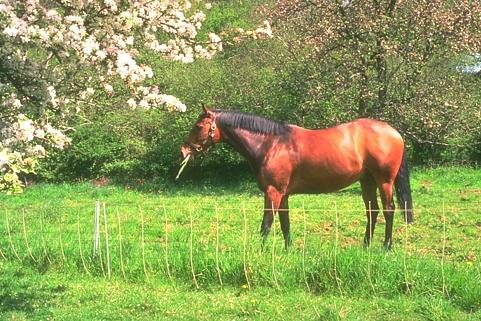
\includegraphics[width=3.5in]{figures/segmentation-scene.jpg}
}
\subfigure[human segmentations of the same scene]{
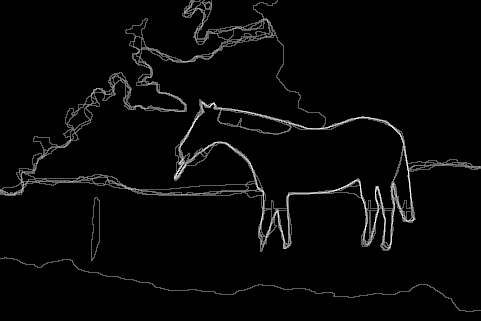
\includegraphics[width=3.5in]{figures/human-segmentations.png}
}
\subfigure[an automated segmentation of the same scene using local image properties (brightness and texture gradients); we see that the automated segmentation fails to capture the holistic understanding of the scene shown in the human segmentations in (b)]{
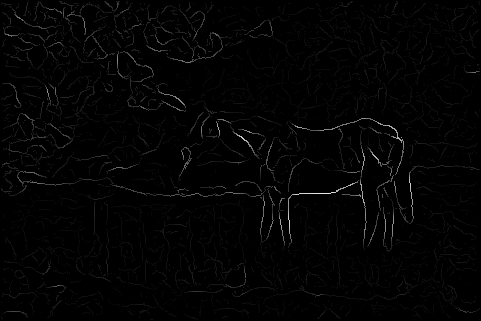
\includegraphics[width=3.5in]{figures/automated-segmentations.png}
}
\caption{Human and automated segmentation performance on an image from the Berkeley Segmentation Dataset~\cite{Martin-2001}.}
\label{fig:segmentation}
\end{figure}
%*******************************************************************************

Image segmentation is challenging because determining if two pixels in an image "go together"~\cite{Szeliski-2010} often requires an abstract and holistic understanding of the image, and in general it is difficult for computer algorithms to gain this understanding. Analyzing local image features such as edges and contours, as well as local image properties such as color and texture is not guaranteed to capture the relevant relationships between pixels (see Figure \ref{fig:segmentation}). Determining the mixture of image properties required to capture such relationships remains an active area of research.

%*******************************************************************************
% FIGURE Medical Image
\begin{figure*}[t]
\centering
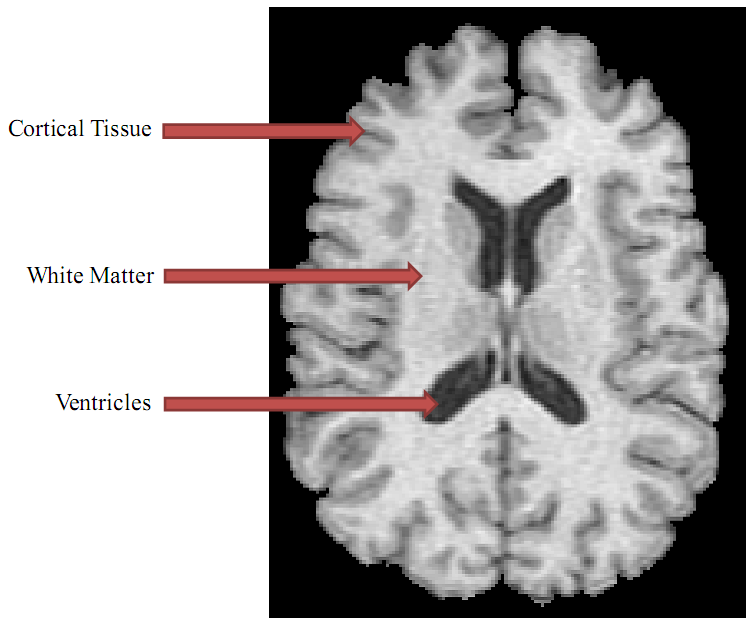
\includegraphics[width=6.0in]{figures/medical-image-with-labels.png}
\caption{A typical 2D cross-sectional magnetic resonance image of a brain. Distinct structures are apparent (labelled with red arrows for additional clarity) but boundaries are not precisely defined~\cite{Pham-1999}.}
\label{fig:medical-image}
\end{figure*}
%*******************************************************************************
%*******************************************************************************
% FIGURE Medical Image
\begin{figure*}[t]
\centering
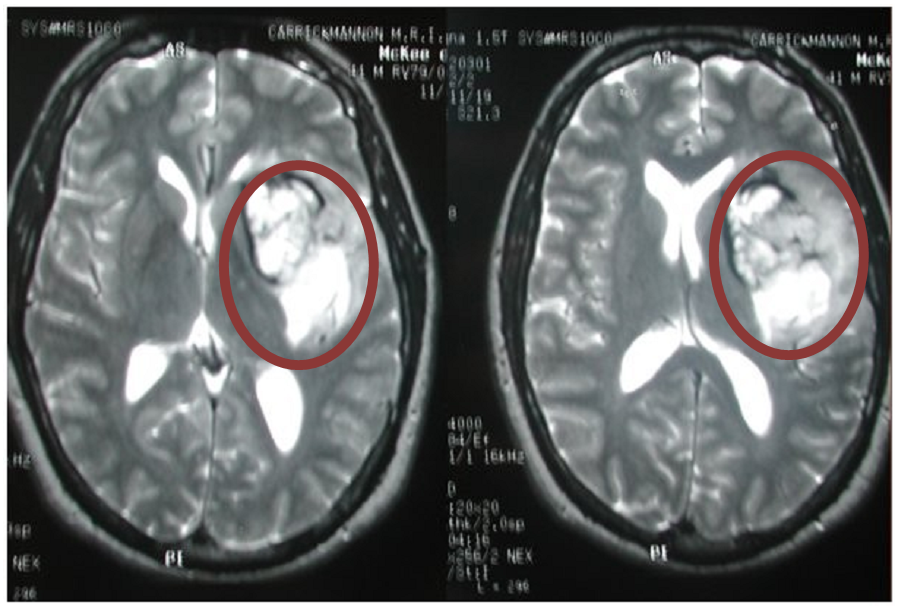
\includegraphics[width=6.0in]{figures/brain-tumour-with-labels.png}
\caption{A 2D cross-sectional magnetic resonance image of a brain with a visible brain tumour. The tumour (approximately outlined in red) is heterogeneous and not precisely defined~\cite{Botchu-2005}.}
\label{fig:brain-tumour}
\end{figure*}
%******************************************************************************
Image segmentation is particularly important in diagnostic medicine. The use of medical scanning equipment to acquire 3D images of the human body is commonplace. These images must be carefully segmented into meaningful regions before they can be be quantified and analyzed for the purposes of diagnosis and treatment planning. For example, there is no single treatment for cancer which is most effective for treating all sizes of tumour. In other words, for different sizes of tumour, there are different treatment methods which offer optimal patient outcomes. To determine the optimal treatment for a particular cancer patient, a physician must often segment a tumour from a medical image to accurately determine its size.

Physicians often resort to very crude approximations when segmenting large 3D medical images since precise manual segmentation of these images is such a slow process. This practice may result in sub-optimal patient outcomes in cases where the physician's segmentation exhibits large approximation error.

In the medical imaging domain, image segmentation is especially challenging since current medical scanning equipment may introduce noise and non-linearly distributed image intensity distortions into the resulting medical images. Moreover, medical images typically lack precisely defined intensity boundaries at physical tissue boundaries (see Figure \ref{fig:medical-image}).

Threshold-based flood-fill techniques~\cite{Chen-2008} can compute  segmentation results very quickly but often fail when the region-of-interest (ROI) is heterogeneous~\cite{Unger-2008}. This makes it difficult to segment some  structures, like brain tumors, which have variable intensity, texture, shape and size~\cite{Chen-2008} (see Figure \ref{fig:brain-tumour}). Computer-assisted level set segmentation techniques~\cite{Lefohn-2003-MICCAI,Cates-2004} have been shown to produce accurate segmentations and reduce the variability of difficult segmentation tasks in medical imaging. The level set method is a powerful, flexible, and accurate numerical technique for image segmentation under challenging conditions since the segmentation process can depend on image properties (e.g. color or texture) and can enforce geometric constraints on the segmented regions (e.g. smoothness).

The level set method begins with an implicitly represented seed surface embedded within a regular scalar grid. The level set method deforms this surface to envelop a corresponding region-of-interest (ROI) in the original image by iteratively solving a partial differential equation defined at each grid element. This method typically requires thousands of iterations to converge and there can be millions of grid elements that must be updated during each iteration. The level set method has historically resulted in long computation times and therefore limited clinical utility.

In response to the demand for faster level set segmentation methods, researchers have developed significantly accelerated algorithms for solving the level set equations~\cite{Whitaker-1994, Adalsteinsson-1995,Peng-1999,Lefohn-2003-Vis,Lefohn-2003-MICCAI,Lefohn-2004,Cates-2004,Jeong-2009}. These algorithms are motivated by the observation that computations can be avoided in regions that are far away from the level set surface without affecting the resulting segmentation. Leveraging this insight, previous algorithms maintain dynamic data structures to represent the \emph{active computational domain} -- the grid elements that must be updated during each iteration. There is significant spatial coherence among these grid elements since they are all near the level set surface.
The fastest algorithms leverage the general-purpose and massively parallel computational power of commodity graphics processing units (GPUs). These parallel GPU algorithms~\cite{Lefohn-2003-Vis,Lefohn-2003-MICCAI,Lefohn-2004,Cates-2004,Jeong-2009} are motivated by the observation that within each iteration, the solution of the level set equations at each grid element is independent from the solution at each other grid element. Therefore the solutions for every grid element can be computed in parallel on the many computational cores of the GPU. However, the previous state-of-the-art GPU algorithm I test in this thesis took over 100 seconds  to converge  on  the  white and grey matter in a $256^3$ medical image of a human head, even when running on a state-of-the-art GPU. The fastest level set segmentation algorithms are still too slow. This limitation constrains clinical applications and motivates the research herein.

In this thesis I present a novel GPU level set segmentation algorithm that dramatically improves computational efficiency without sacrificing segmentation accuracy. In a series of controlled experiments using noisy magnetic resonance images (MRIs) generated from the BrainWeb Simulated Brain Database~\cite{BrainWeb-2010,Kwan-1996,Cocosco-1997,Collins-1998,Kwan-1999}, I demonstrate that my algorithm reduces the total number of processed grid elements by $16 \times$ and converges $14 \times$ faster than previous state-of-the-art GPU algorithms~\cite{Lefohn-2003-Vis,Lefohn-2003-MICCAI,Lefohn-2004,Cates-2004} with equal accuracy in all experiments. My algorithm runs entirely on the GPU without requiring any additional data processing on the CPU, thereby enabling interactive 3D visualization and real-time control of the evolving segmentation.

\section{Assumptions}

Given the acknowledged difficulty of fully automated image segmentation, researchers have focused on easier sub-problems in order to obtain results that are competitive with human segmentations~\cite{Szeliski-2010}. In this thesis I tackle a simpler sub-problem of the more general image segmentation problem by making the following assumptions:

\begin{itemize}

    \item I assume that my algorithm is only concerned with generating binary (i.e. foreground and background) segmentations. This assumption is motivated by a common workflow in the medical community: segmenting a region-of-interest (ROI) from a medical image for subsequent analysis.

    \item I assume that my algorithm is guided by user interaction. This assumption is motivated by a common preference the medical community: physicians often prefer intuitive interactive segmentation methods over fully automated methods~\cite{Unger-2008} since interactive methods allow them to drive the segmentation process according to their domain expertise. This expertise would be difficult to distill into a fully automated method.

    \item I assume that there is some difference in image intensity between foreground and background objects. Moreover I assume that this difference approximately exceeds the heterogeneity of the foreground objects being segmented and the noise in the image. Previous state-of-the-art GPU level set segmentation algorithms~\cite{Lefohn-2003-Vis,Lefohn-2003-MICCAI,Lefohn-2004,Cates-2004,Jeong-2009} also make this assumption as it simplifies the solution of the level set equations. In practice this assumption does not always hold, and therefore it introduces a limitation that my algorithm shares with previous GPU algorithms~\cite{Lefohn-2003-Vis,Lefohn-2003-MICCAI,Lefohn-2004,Cates-2004,Jeong-2009}. This assumption could be relaxed with a more intelligent accounting of image properties when solving the level set equations. However this is not the focus of my research. Instead I am focused on developing optimizations that are orthogonal to the accounting of image properties used when solving the level set equations. The optimizations that I present in this thesis are compatible with a wide variety of image properties and features. 
\end{itemize}

\section{Contributions and Results}

This thesis makes the following contributions:

\begin{itemize}

    \item A novel algorithm for limiting the active computational domain to the minimal set of changing level set grid elements by leveraging both spatial and temporal coherence in the active computational domain;

    \item A formal derivation of the above algorithm;
    
    \item A novel mapping of this algorithm to massively parallel GPU hardware. This GPU algorithm scales efficiently to an unbounded number of parallel processors while performing asymptotically no more work than the most efficient sequential algorithm, and does so in asymptotically fewer steps. This GPU algorithm does not require any additional data processing on the CPU, thereby enabling smooth interactive 3D visualization and real-time control of the evolving segmentation;

    \item A\ formal proof of the above GPU algorithm's asymptotic properties;
and
    \item A series of controlled experiments using noisy magnetic resonance images (MRIs) generated from the BrainWeb Simulated Brain Database~\cite{BrainWeb-2010,Kwan-1996,Cocosco-1997,Collins-1998,Kwan-1999}. I demonstrate significant performance benefits over previous state-of-the-art parallel algorithms~\cite{Lefohn-2003-MICCAI,Lefohn-2003-Vis,Cates-2004,Lefohn-2004}. I demonstrate that my algorithm: reduces the total number of processed level set field elements by $16 \times$ and converges $14 \times$ faster than previous state-of-the-art parallel algorithms; converges $685 \times$ faster than previous sequential algorithms; and produces equally accurate segmentations to previous parallel algorithms with less than 0.2\% variability in all experiments.



\end{itemize}

\section{Thesis Overview}

The remainder of this thesis is organized as follows. In Chapter \ref{chapter:background} I describe the technical background and related work most relevant to my research. I discuss an emerging research field that seeks to accelerate general-purpose parallel computations by performing them on GPUs. I describe the current state-of-the-art GPU algorithms for level set segmentation. I show that previous algorithms maintain a sparse active computational domain that is coherent in space only.

In Chapter \ref{chapter:temporal} I present a new algorithm for maintaining a sparse active computational domain for solving the level set equations that is coherent in both space and time. I provide the intuitive motivation for this algorithm, a discussion of the underlying mathematics, and sequential psuedo-code for clarity.

In Chapter \ref{chapter:parallel} I discuss the challenges associated with parallelizing the algorithm described in the previous chapter. I present a massively parallel algorithm that overcomes these challenges and I discuss an implementation of this algorithm on a commodity GPU.

In Chapter \ref{chapter:evaluation} I describe a methodology for evaluating the parallel algorithm from the previous chapter. I analyze the asymptotic performance and memory efficiency of this algorithm, and describe a series of experiments that compares the computational efficiency and accuracy of my GPU algorithm to a previous state-of-the-art GPU algorithm. The results of these experiments show that my algorithm significantly outperforms the previous state-of-the-art algorithm with no reduction in segmentation accuracy.

In Chapter \ref{chapter:conclusions} I propose future research directions that build on the work presented in this thesis.



\fancyhead[RO,LE]{\thepage}
\fancyfoot{} 
\chapter{Technical Background and Related Work}
\label{chapter:background}

In this chapter I describe the technical background and related work most relevant to my research. I begin this chapter  by discussing an emerging research field that seeks to accelerate general-purpose computations by performing them on GPUs. I motivate the use of GPUs for general-purpose computation with a discussion of their performance advantages. I introduce the \emph{stream programming model} -- an abstract programming model used to design massively parallel algorithms suitable for execution on the GPU. I introduce a set of mathematical tools used to analyze the asymptotic performance of algorithms expressed in the stream programming model. I also discuss two fundamental stream operations that are required in my research. The first operation is known as \emph{all-prefix-sums} (sometimes referred to as \emph{scan}) and involves computing the sum of all elements prior to each element in an input array. The second operation is known as \emph{stream compaction} and involves removing unwanted elements from an input array. I show that stream compaction can be trivially  implemented in terms of all-prefix-sums. I conclude this chapter by describing the current state-of-the-art algorithms for GPU level set segmentation, as well as a CPU level set segmentation algorithm that influenced my research.

%*******************************************************************************
% FIGURE Technology Trends
\begin{figure}[t]
\centering
\subfigure[]{
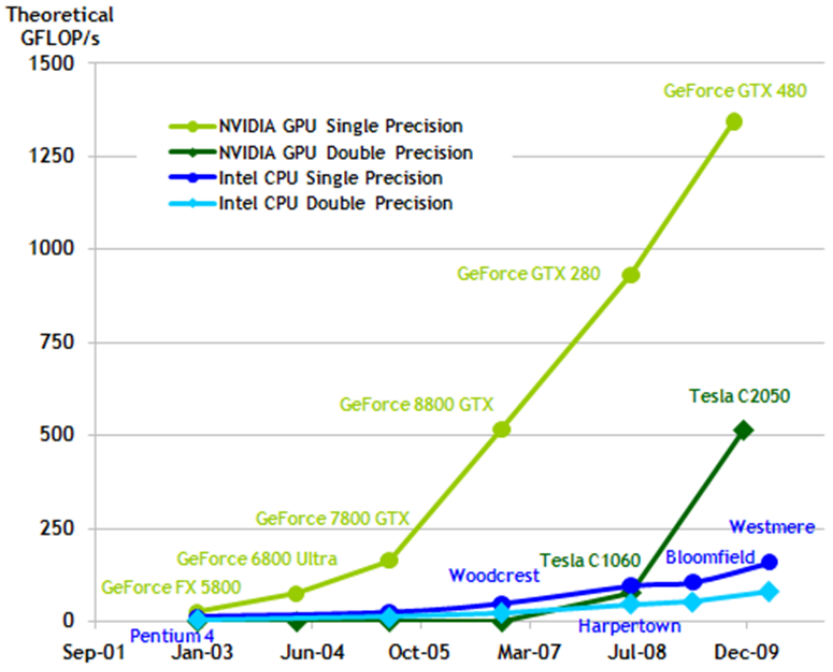
\includegraphics[width=4.0in]{figures/gflops.png}
}
\subfigure[]{
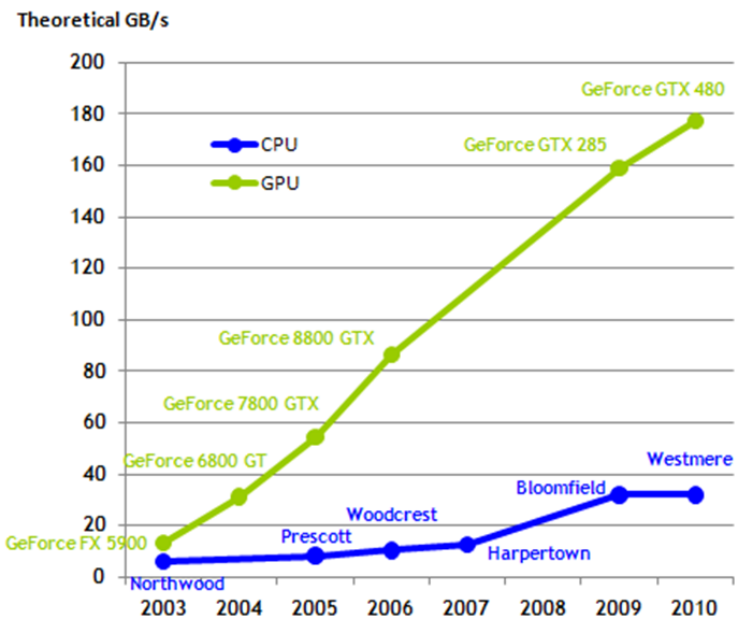
\includegraphics[width=4.0in]{figures/bandwidth.png}
}
\caption{Performance trends for GPUs and CPUs as indicated by floating-point operations per second (GFLOPS) (a) and memory bandwidth (GB/sec) (b)~\cite{NVIDIACUDA-2010}.}
\label{fig:gpu-cpu-performance}
\end{figure}
%*******************************************************************************

\section{General-Purpose Computation on GPUs}

\subsection{GPUs are Powerful, Inexpensive, and Massively Parallel}
In the most comprehensive survey to date relating to general-purpose computation on the GPU~\cite{Owens-2007} -- an emerging research field known as \emph{GPGPU} -- Owens et al.\ write that "GPUs are probably the most powerful computational hardware for the dollar"~\cite{Owens-2007}. Owens et al.\ argue,
\begin{quote}
"graphics architectures provide tremendous provide tremendous memory bandwidth and computational horsepower. For example, the flagship NVIDIA GeForce 7900 GTX (\$378 as of October 2006) boasts 51.2 GB/sec memory bandwidth; the similarly priced ATI Radeon X1900 XTX can sustain a measured 240 GFLOPs, both measured with GPUBench~\cite{Buck-2004}. Compare to 8.5 GB/sec and 25.6 GFLOPS theoretical peak for the SSE units of a dual-core 3.7 GHz Intel Pentium Extreme Edition 965~\cite{Intel-2006}."~\cite{Owens-2007}
\end{quote}

Owens et al.\ go on to argue,
\begin{quote}
"graphics hardware is fast and getting faster quickly. For example, arithmetic throughput (again measured by GPUBench) of NVIDIA's current-generation launch product, the GeForce 7800 GTX (165 GFLOPS), more than triples that of its predecessor, the GeForce 6800 Ultra (53 GFLOPS). In general the computational capabilities of GPUs, measured by the traditional metrics of graphics performance, have compounded at an average yearly rate of 1.7 (pixels/second) to 2.3 (vertices/second). This rate of growth significantly outpaces the often-quoted Moore's Law as applied to traditional microprocessors; compare to a yearly rate of roughly 1.4 for CPU performance~\cite{Ekman-2005}."~\cite{Owens-2007}  
\end{quote}

The technology trends Owens et al.\ discuss are shown in Figure \ref{fig:gpu-cpu-performance}.

In addressing the question of why GPU performance increases faster than CPU performance, Owens et al.\ write,
\begin{quote}
"semiconductor capability, driven by advances in fabrication technology, increases at the same rate for both [CPU and GPU] platforms. The disparity can be attributed to fundamental architectural differences: CPUs are optimized for high performance on sequential code, with many transistors dedicated to extracting instruction-level parallelism with techniques such as branch prediction and out-of-order execution. On the other hand, the highly data-parallel nature of graphics computations enables GPUs to use additional transistors more directly for computation, achieving higher [computational throughput] with the same transistor count."~\cite{Owens-2007}
\end{quote}

GPUs take advantage of the abundant data parallelism in computer graphics by concurrently processing data elements on a large number of parallel cores. For example NVIDIA's current flagship GPU in August 2010, the NVIDIA GeForce GTX 480, contains 512 parallel computational cores~\cite{NVIDIAGeForceGTX480-2010}. Moreover the number of parallel computational cores on NVIDIA\ GPUs has roughly doubled every year for the last three years~\cite{NVIDIAGeForce9800-2010,NVIDIAGeForceGTX280-2010,NVIDIAGeForceGTX480-2010}. This trend is likely to continue for at least the next decade. This is because the number of transistors per die on GPUs is likely to double each year for at least the next decade~\cite{Owens-2005}, and for much longer there will likely be enough data parallelism in computer graphics to increase effective performance by adding computational cores. From the arguments above, we see that the GPU is a powerful, inexpensive, and massively parallel processor.

\subsection{Writing General-Purpose GPU Programs Using the Stream Programming Model}

Until very recently the computational power of the GPU was only available  through graphics APIs like OpenGL, DirectX, and their corresponding languages for describing geometric and optical properties of surfaces -- known as \emph{shading languages}. In order to solve non-graphics problems using GPUs, programmers were historically required to cast the computations in terms of graphics primitives. Of this programming model, Owens et al.\ write, 
\begin{quote}
"more often than not, the graphics-centric nature of shading languages makes GPGPU programming more difficult than it needs to be. As a simple example, initiating a GPGPU computation usually involves drawing a primitive. Looking up data from memory is done by issuing a texture fetch. The GPGPU program may conceptually have nothing to do with drawing geometric primitives and fetching textures, yet the shading languages described in the previous section force the GPGPU application writer to think in terms of geometric primitives [...] and textures. Instead, GPGPU algorithms are often best described as memory and math operations, concepts much more familiar to CPU programmers."~\cite{Owens-2005}
\end{quote}

Fortunately it is now possible to write general purpose programs that execute in parallel on the GPU without needing to awkwardly cast the computations in terms of graphics primitives. Instead, new GPU programming languages allow data parallel algorithms to be expressed in the more abstract \emph{stream programming model}. This programming model inherently structures algorithms in a way that expresses abundant data parallelism and transparently scales performance with the number of available parallel computational cores. The stream programming model is well suited to express data parallel algorithms in a way that can be efficiently mapped to massively parallel GPU hardware.

Owens describes the stream programming model,
\begin{quote}
"In the stream programming model, all data is represented as a \emph{stream}, which we define as an ordered set of data of the same data type. That data type can be simple (a stream of integers or floating-point numbers) or complex (a stream of points or triangles or transformation matrices). While a stream can be any length, we will see that operations on streams are most efficient if streams are long (hundreds or more elements in a stream). Allowed operations on streams include copying them, deriving substreams from them, indexing into them with a separate index stream, and performing computation on them with \emph{kernels}.

A kernel operates on entire streams, taking one or more streams as inputs and producing one or more streams as outputs. The defining characteristic of a kernel is that it operates on entire streams  of elements as opposed to individual elements. The most typical use of a kernel is to evaluate a function on each element of an input stream; for example, a transformation kernel may project each element of a stream of points into a different coordinate system. Other desirable kernel operations include expansions (in which more than one output element is produced for each input element), reductions (in which more than one element is combined into a single output element), or filters (in which a subset of input elements are output).

Kernel outputs are functions only of their kernel inputs, and within a kernel, computations on one stream element are never dependent on computations on another element. These restrictions have two major advantages. First, the data required for kernel execution is completely known when the kernel is written (or compiled). Kernels can thus be highly efficient when their input elements and their intermediate computed data are stored locally  or are carefully controlled global references. Second, requiring independence of computation on separate stream elements within a single kernel allows mapping what appears to be a serial kernel calculation onto data-parallel hardware.

In the stream programming model, applications are constructed by chaining multiple kernels together."~\cite{Owens-2005}
\end{quote}
%*******************************************************************************
\begin{Listing}[t]
    \caption{High level parallel pseudo-code for computing the $n$-dimensional vector $R$ as the sum of the two $n$-dimensional vectors $A$ and $B$. A subscript notation is used to denote individual vector elements. For example $R_{i}$ refers to the $i^{th}$ element of $R$.}
    \begin{algorithmic}[1]
        \FORALL { $ i \gets 0 \mbox{ to } n \mbox{ \ in parallel}$ } 
            \STATE { $ R_{i} \gets A_{i} +B_{i} $ }
        \ENDFOR
    \end{algorithmic}
    \label{alg:high-level-vector-add}
\end{Listing}
%*******************************************************************************
%*******************************************************************************
\begin{Listing}[t]
    \caption{Expressing the high-level parallel pseudo code from Listing \ref{alg:high-level-vector-add} as a stream program. Note that the \textbf{VectorAdd} kernel is written as though it is only processing a single element. The computation in this kernel is implicitly mapped to all stream elements and performed in parallel on the stream processor.}
    \scriptsize
    \begin{verbatim}
// this kernel adds two N-dimensional vectors in parallel
kernel VectorAdd( stream result<>, stream int a<>, stream int b<> )
{
    result = a + b;
}

// this program adds two N-dimensional vectors together in parallel 
void main()
{
    // define int arrays in main memory
    int a[N], int b[N];
    
    // define int streams on the stream processor
    stream int sA<N>, sB<N>, sResult<N>;
 
    // ... initialize the input arrays ...
    
    // ... copy the contents of the input arrays into the input streams ...
        
    // invoke the VectorAdd kernel
    VectorAdd( sResult, sA, sB );

    // ... at this point sResult contains the results of the vector addition ...
}
    \end{verbatim}
    \label{alg:stream-program-vector-add}
\end{Listing}
%*******************************************************************************
Listing \ref{alg:high-level-vector-add} shows high level parallel pseudo-code for adding two $n$-dimensional vectors, and Listing \ref{alg:stream-program-vector-add} shows how this pseudo-code would be expressed as a stream program.

\subsection{Asymptotic Complexity}

We are often interested in analyzing the efficiency of algorithms independently from the performance characteristics of the machine on which they are executing. Rather than directly measuring number of operations an algorithm performs for a particular input, we determine the amount of work an algorithm performs, and the amount of memory it consumes, as a function of input size for arbitrarily large inputs.
We refer to this abstract measure of efficiency as an algorithm's \emph{asymptotic} complexity.

\subsection{Analyzing the Asymptotic Complexity of Stream Algorithms}

To analyze the asymptotic behavior of sequential algorithms, we assume the algorithm executes on a theoretical processor that performs one canonical unit of work per unit of time. This theoretical computational model is known as the random access machine (RAM) model, and the theoretical processor is known as a RAM processor.~\cite{Atallah-1998}

Analyzing the asymptotic behavior of parallel algorithms requires us to extend this model. Again our goal is to analyze the parallel algorithm independently from the physical system on which it is running. Therefore in our extended theoretical computational model, we assume there are an unbounded number of RAM processors and that all these processors share a common memory. This is known as the \emph{\emph{parallel random access machine}} (PRAM) model, and the parallel processors are known as PRAM processors.~\cite{Atallah-1998}

In the RAM model, the amount of work a sequential algorithm performs is equal to the amount of time it takes to execute. In the PRAM model, this is equality does not hold in general, since more than one processor may be doing a unit of work in a unit of time. Therefore determining the asymptotic runtime complexity of parallel algorithms involves deriving expressions for two important quantities. The first quantity is known as \emph{work-complexity}, which refers to the total amount of work performed by the parallel algorithm~\cite{Atallah-1998}. The second quantity is known as \emph{step-complexity}, which refers to the total number of steps (i.e. units of time) required for the parallel algorithm to execute, given the unbounded number of processors in the PRAM model~\cite{Nyland-2000}.

A parallel algorithm is \emph{work-efficient} if it performs asymptotically no more work than the most efficient sequential algorithm. In practice it is important for parallel algorithms to be work-efficient. If a parallel algorithm is not work-efficient, and it is executed on a machine with a finite number of processors, then the most efficient sequential algorithm will outperform the parallel algorithm on sufficiently large inputs.~\cite{Atallah-1998}

A parallel algorithm is \emph{step-efficient} if it requires asymptotically fewer steps to execute than the most efficient sequential algorithm. It is important for parallel algorithms to be step-efficient. If a parallel algorithm is not step-efficient, there is no asymptotic benefit to using the parallel algorithm over the most efficient sequential algorithm.

\phantomsection
\subsection{All-Prefix-Sums}
\phantomsection

The \emph{all-prefix-sums} operation, also known as \emph{scan}, is one of the most important primitive operations for constructing data parallel algorithms. All-prefix-sums involves computing, for every element of an input array, the sum of all the previous elements in the array. All-prefix-sums can be used to implement efficient parallel algorithms for quick-sort, radix-sort, sparse matrix multiplication, removing marked elements from arrays, parsing strings into tokens, lexicographic sorting, constructing data structures for fast image filtering, and many other fundamental tasks~\cite{Blelloch-1993,Hensley-2005}. In particular, all-prefix-sums is an important primitive operation in the parallel level set segmentation algorithm described in Chapter \ref{chapter:parallel}, since this algorithm requires an efficient parallel method for removing marked elements from arrays.

\begin{samepage}
For the purposes of this thesis, I define all-prefix-sums as follows:
\begin{quote}
Given the following input array of size $n$,
\end{quote}
\begin{equation}
\left[ a_0 , a_1 , a_2 , \ldots , a_n \right]
\end{equation}
\begin{quote}
all-prefix-sums returns the following array as output,
\end{quote}
\begin{equation}
\left[0,a_0,\left(\sum_{ i = 0 }^{ 1 } a_i\right),\left(\sum_{ i = 0 }^{ 2 } a_i\right),\left(\sum_{ i = 0 }^{ 3 } a_i\right),\ldots,\left(\sum_{ i = 0 }^{ n-1 } a_i\right)\right]
\end{equation}
\begin{quote}
For example, if the input array was $[10, 4, 6, 8, 4, 3, 2, 5]$, the output of all-prefix-sums would be the array $[0,10,14,20,28,32,35,37]$.
\end{quote}
\end{samepage}

%*******************************************************************************
\begin{Listing}[t]
    \caption{Sequential pseudo-code for computing all-prefix-sums of an input array $A$ and storing the results in an output array $R$. A subscript notation is used to denote individual array elements. For example $R_{i}$ refers to the $i^{th}$ element of $R$. }
    \begin{algorithmic}[1]
        \STATE { $ R_0 \gets 0 $ }
        \FOR { $ i \gets 1 \mbox{ to } n $ } 
            \STATE { $ R_{i} \gets R_{ i - 1 } + A_{i} $ }
        \ENDFOR
    \end{algorithmic}
    \label{alg:sequential-all-prefix-sums}
\end{Listing}
%*******************************************************************************

A trivial sequential algorithm for all-prefix-sums is shown in Listing \ref{alg:sequential-all-prefix-sums}. I note that this algorithm performs $O(n)$ work. This algorithm cannot be parallelized straight-forwardly since each iteration of the \textbf{for} loop in Listing \ref{alg:sequential-all-prefix-sums} depends on the previous iteration. Sengupta et al.\ discuss the challenges involved in parallelizing all-prefix-sums,

\begin{quotation}
"How do we compute the value of the last element in the output? That value is a function of \emph{every} value in the input stream. With a serial processor, such a computation is trivial, but with a parallel processor, it is more difficult. The naive way to compute each output in parallel is for every element in the output stream to sum all preceding values from the input stream. This approach requires $O(n^2)$ total memory accesses and addition operations. This cost is too high."~\cite{Sengupta-2007}
\end{quotation}

Blelloch introduced a work-efficient and step-efficient parallel algorithm for all-prefix-sums that avoids the costs of the naive algorithm~\cite{Blelloch-1993}. He also discussed all-prefix-sums in the context of several important data parallel applications~\cite{Blelloch-1993}. Horn introduced the first GPU algorithm for all-prefix-sums as part of a collision-detection application~\cite{Horn-2005}. Hensley et al.\ improve on the performance of Horn's GPU implementation in their work on fast image filtering~\cite{Hensley-2005}. Although these GPU algorithms are step-efficient, they are not work-efficient. This inefficiency has a significant impact on practical performance, especially for large arrays. Sengupta et al.\ and Gre\ss \ et al.\ each describe work-efficient GPU algorithms for all-prefix-sums~\cite{Sengupta-2006,Greb-2006}. Harris et al.~\cite{Harris-2007}, Dotsenko et al.~\cite{Dotsenko-2008}, and Sengupta et al.~\cite{Sengupta-2011} improve on the performance of these GPU algorithms and preserve their asymptotic properties.~\cite{Sengupta-2007}

Harris et al.\ provide a high-level description of the work-efficient GPU all-prefix-sums algorithm used in this thesis,
\begin{quotation}
"We would like to find an algorithm that would approach the efficiency of the sequential algorithm, while still taking advantage of the parallelism in the GPU. Our goal in this section is to develop a work-efficient scan algorithm [...] based on the one presented by Blelloch~\cite{Blelloch-1993}. To do this we will use an algorithmic pattern that arises often in parallel computing: balanced trees. The idea is to build a balanced binary tree on the input data and sweep it to and from the root to compute the prefix sum. A binary tree with $n$ leaves has $d = \log_2n$ levels, and each level $d$ has $2^d$ nodes. If we perform one add per node, then we will perform $O(n)$ adds on a single traversal of the tree."
\end{quotation}

In other words, if we perform one operation per node for a balanced binary tree with $n$ leaves, then we will have performed a total of $2n - 1$ operations. Therefore each time we sweep across the entire tree performing one operation per node, we will have performed $O(n)$ operations.
Harris et al. goes on to describe this concept of distributing work across a balanced binary tree in more detail,
\begin{quotation}
"The tree we build is not an actual data structure, but a concept we use to determine what each thread does at each step of the traversal. The algorithm consists of two phases: the up-sweep phase and the down-sweep phase. In the up-sweet phase, we traverse the tree from leaves to root computing partial sums at internal nodes of the tree, as shown in Figure \ref{fig:upsweep}. Pseudo-code for the up-sweep phase is given in Listing \ref{alg:all-prefix-sums-upsweep}.

In the down-sweep phase, we traverse back down the tree from the root, using the partial sums from the reduce phase to build the scan in place on the array. We start by inserting zero at the root of the tree, and on each step, each node at the current level passes its own value to its left child, and the sum of its value and the former value of its left child to its right child. The down-sweep is shown in Figure \ref{fig:downsweep}, and pseudo-code is given in Listing \ref{alg:all-prefix-sums-downsweep}."~\cite{Harris-2007}
\end{quotation}

In principle this all-prefix-sums algorithm sweeps twice across a balanced binary tree with $n$ leaves. Therefore it performs $O(n)$ work. The operations at each level of the tree are independent, and can therefore be performed in parallel in a single step. Since there are $\log_2 n$ levels in the tree, each sweep across the tree requires $O(\log_2 n)$ steps. Therefore this all-prefix-sums algorithm is both work-efficient and step-efficient.
\pagebreak
%*******************************************************************************
% Upsweep
\begin{figure*}[t]
\centering
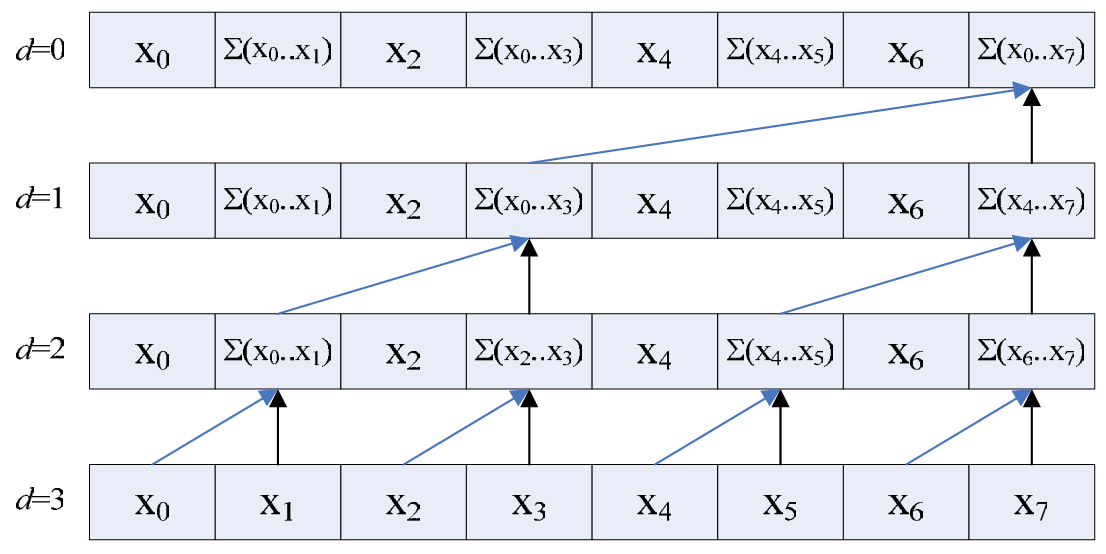
\includegraphics[width=6.0in]{figures/upsweep.png}
\caption{The up-sweep phase of the work-efficient parallel \emph{all-prefix-sums} algorithm used in this thesis~\cite{Blelloch-1993,Harris-2007,Sengupta-2011}. Each row $d$ refers to one step of the up-sweep algorithm. The bottom row ($d=3$) is the input list. The up-sweep algorithm begins at the leaf nodes ($d=3$) and proceeds up the tree to the root ($d=0$). Pseudo-code for this algorithm is given in Listing \ref{alg:all-prefix-sums-upsweep}.}
\label{fig:upsweep}
\end{figure*}
%*******************************************************************************
%*******************************************************************************
\begin{Listing}[t]
    \caption{Parallel pseudo-code for the up-sweep phase of the work-efficient parallel \emph{all-prefix-sums} algorithm used in this thesis. The input is an array $A$ of size $n$. The output is written in-place in $A$. After this up-sweep phase has completed, $A$ must undergo the down-sweep phase given in Listing \ref{alg:all-prefix-sums-downsweep}. After this down-sweep phase, $A$ will contain the final output of the all-prefix-sums operation. A subscript notation is used to denote individual array elements. For example $A_{i}$ refers to the $i^{th}$ element of $A$.~\cite{Blelloch-1993} }
    \begin{algorithmic}[1]
        \FOR { $ d \gets \log_2(n) - 1 \mbox{ down to } 0$ } 
            \STATE { $ k \gets \log_2(n) - d $ } 
            \FORALL { $ i \gets 0 \mbox{ to } n-1  \mbox{ \ incrementing by } 2^{k} \mbox{ \ in parallel } $ } 
                \STATE { $ A_{i + 2^{k}-1} \gets A_{i + 2^{k-1}-1} + A_{i + 2^{k}-1} $ }
            \ENDFOR
        \ENDFOR
    \end{algorithmic}
    \label{alg:all-prefix-sums-upsweep}
\end{Listing}
%*******************************************************************************
\clearpage
%*******************************************************************************
% Downsweep
\begin{figure*}[t]
\centering
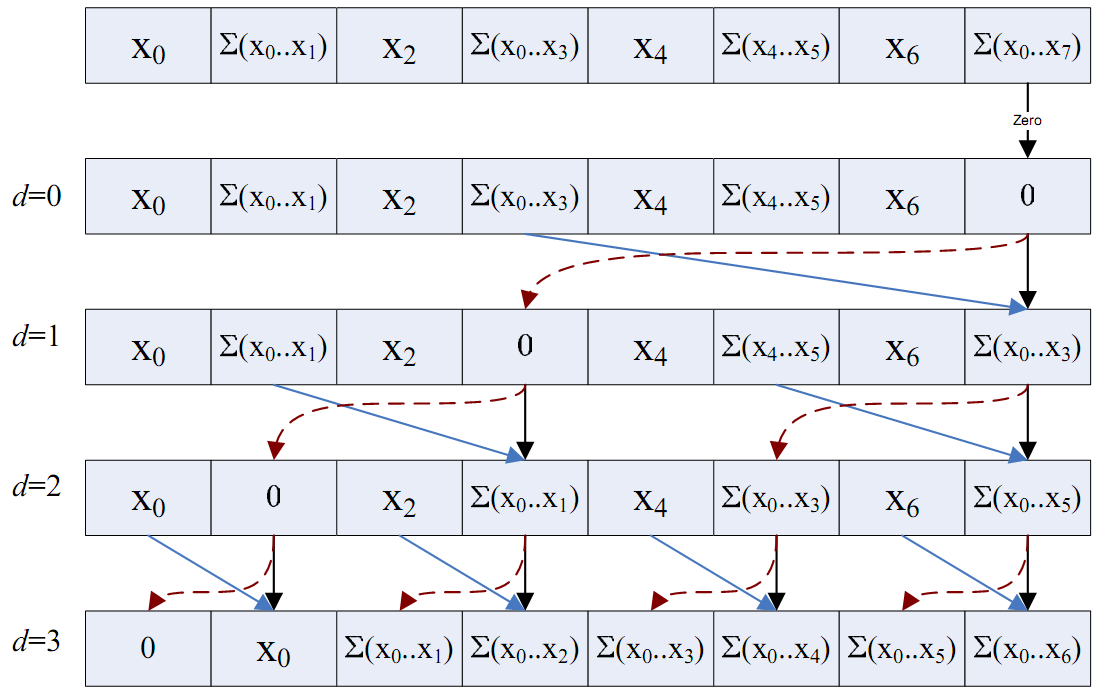
\includegraphics[width=6.0in]{figures/downsweep.png}
\caption{The down-sweep phase of the work-efficient parallel \emph{all-prefix-sums} algorithm used in this thesis~\cite{Blelloch-1993,Harris-2007,Sengupta-2011}. Each row $d$ refers to one step of the down-sweep algorithm. The top row is given by the results of the up-sweep algorithm shown in Figure \ref{fig:upsweep}. The down-sweep algorithm begins at the root node of the tree ($d=0$) and proceeds down the tree to the leaf nodes ($d=3$). Pseudo-code for this algorithm is given in Listing \ref{alg:all-prefix-sums-downsweep}}
\label{fig:downsweep}
\end{figure*}
%********************************************************************************
%********************************************************************************
\begin{Listing}[h]
    \caption{Parallel pseudo-code for the down-sweep phase of the work-efficient parallel \emph{all-prefix-sums} algorithm  used in this thesis. The input is an array $A$ of size $n$ that has undergone the up-sweep phase given in Listing \ref{alg:all-prefix-sums-upsweep}. The output is written in-place in $A$. After this algorithm has completed, $A$ will contain the final output of the \emph{all-prefix-sums} operation. A subscript notation is used to denote individual array elements. For example $A_{i}$ refers to the $i^{th}$ element of $A$.~\cite{Blelloch-1993}}
    \begin{algorithmic}[1]
        \STATE{ $ A_{n-1} \gets 0$ }
        \FOR { $ d \gets 1 \mbox{ to } \log_2(n) - 1 $ }
            \STATE{ $ k \gets \log_2(n) - d$
            \FORALL { $ i \gets 0 \mbox{ to } n - 1 \mbox{ \ incrementing by } 2^{k} \mbox{ \ in parallel } $ } 
                \STATE { $ t \gets A_{i + 2^{k-1}-1}$ }
                \STATE { $ A_{i + 2^{k-1}-1} \gets A_{i + 2^{k}-1} $ }
                \STATE { $ A_{i + 2^{k}-1} \gets t + A_{i + 2^{k}-1} $ }
            \ENDFOR
        \ENDFOR
    \end{algorithmic}
    \label{alg:all-prefix-sums-downsweep}
\end{Listing}
%********************************************************************************
\clearpage
\subsection{Stream Compaction}
Removing unwanted elements from a data stream -- an operation known as \emph{stream compaction} -- is an important task in many parallel algorithms~\cite{Blelloch-1993,Horn-2005,Ziegler-2006,Billeter-2009}, including the parallel level set segmentation algorithm described in Chapter \ref{chapter:parallel}. Given a data array and a flag array that indicates which elements should be kept from the data array, the stream compaction operation returns a dense array of all the elements from the data array that were marked for retention, with none of the elements that were marked for deletion.
\begin{samepage}
For the purposes of this thesis, I define the stream compaction operation as follows:
\begin{quote}
Given the following input data array $A$ of size $n$,
\end{quote}
\begin{equation}
\left[ a_0 , a_1 , a_2 , \ldots , a_n \right]
\end{equation}
\begin{quote}
and an input flag array $F$ of size $n$,
\end{quote}
\begin{eqnarray}
\left[ f_0 , f_1 , f_2 , \ldots , f_n \right] & \mbox{ where } & \forall_{0 \leq i \leq n} : f_i \in \{\mbox{\textbf{remove}},\mbox{\textbf{keep}}\} &
\end{eqnarray}
\begin{quote}
I define a list of size $k \leq n$,
\end{quote}
\begin{eqnarray}
[l_0,l_1,l_2,\ldots,l_k] & \mbox{ where } & \forall_{0 \leq i \leq k} : f_{l_i} = \mbox{\textbf{keep}} \\
& & \forall_{ j : f_j = \mbox{\textbf{keep}} }: \exists_{ 0 \leq i \leq k } : j=l_i \\
& & \forall_{0 \leq i,j \leq k} : {l_i} = l_j \equiv i=j \\
& & \forall_{0 \leq i,j \leq k} : {l_i} < l_j \equiv i < j
\end{eqnarray}
\begin{quote}
The stream compaction operation returns the array,
\end{quote}
\begin{equation}
\left[ a_{l_0} , a_{l_1} ,a_{l_2} , \ldots , a_{l_k} \right]
\end{equation}
\begin{quote}
For example, if the input data array was $[10, 4, 6, 8, 4, 3, 2, 5]$, and the input flag array was $[0,1, 1, 1, 0, 0, 1, 0]$ where $0=\mbox{\textbf{remove}}$ and $1=\mbox{\textbf{keep}}$, the output of compact operation would be the array $[4,6,8,2]$.
\end{quote}
\end{samepage}

The conditions on the list $L$ warrant a more detailed discussion. The first condition specifies that all the entries in $L$ correspond to the index of some \textbf{keep} entry in $F$. The second condition specifies that the indices of all \textbf{keep} entries in $F$ correspond to some entry in $L$. The third condition specifies that there are no repeated entries in $L$. The fourth condition specifies that the entries in $L$ are in ascending order. Together these conditions specify that all the entries in $A$ that are marked for retention, and no others, will be in the output array exactly once with their relative ordering preserved. 
%*******************************************************************************
\begin{Listing}[t]
    \caption{Sequential pseudo-code for compacting an input data array $A$ based on an input flag array $F$ that indicates which elements should be kept. The compacted result is written into the output array $R$. A subscript notation is used to denote individual array elements. For example $R_{i}$ refers to the $i^{th}$ element of $R$. }
    \begin{algorithmic}[1]
        \STATE { $ c \gets 0 $ }
        \FOR { $ i \gets 0 \mbox{ to } n-1 $ } 
            \IF{ $F_i = \mbox{keep}$ }
                \STATE { $ R_{c} \gets A_{ i }$ }
                \STATE { $ c \gets c + 1$ }                
            \ENDIF
        \ENDFOR
    \end{algorithmic}
    \label{alg:compaction-sequential}
\end{Listing}
%*******************************************************************************
%*******************************************************************************
\begin{Listing}[t]
    \caption{Parallel pseudo-code for compacting an input data array $A$ based on an input flag array $F$ that indicates which elements should be kept. A value of 0 in $F$ means remove and a value of 1 in $F$ means keep. The compacted result is written into the output array $R$. A subscript notation is used to denote individual array elements. For example $R_{i}$ refers to the $i^{th}$ element of $R$. }
    \begin{algorithmic}[1]
        \STATE { $ S \gets \mbox{\textbf{all\_prefix\_sums}}(F) $ }
        \FOR { $ i \gets 0 \mbox{ to } n-1 \mbox{ \ in parallel } $ } 
            \IF{ $F_i = 1$ }
                \STATE { $ R_{S_i} \gets A_{ i }$ }
            \ENDIF
        \ENDFOR
    \end{algorithmic}
    \label{alg:compaction-parallel}
\end{Listing}
%*******************************************************************************

A sequential algorithm for stream compaction is given in Listing \ref{alg:compaction-sequential}. Like all-prefix-sums, a sequential algorithm for stream compaction is trivial but cannot be parallelized straight-forwardly because each loop iteration depends on the previous iteration. It is easy enough for each thread to independently decide if it should keep an element of an input stream. However if a thread does decide to keep an element, it is difficult for the thread to determine where it should write this element in the output array. Determining the correct location for each output element depends on results of all the other output elements. 

Blelloch used all-prefix-sums to solve the problem of efficiently determining the correct location of each output element~\cite{Blelloch-1993}. The most efficient GPU stream compaction algorithms~\cite{Dotsenko-2008,Sengupta-2011}, including the one used in this thesis~\cite{Sengupta-2011}, are directly inspired by Blelloch's algorithm. In this sense, we see the deep connection between stream compaction and all-prefix-sums. 

Blelloch's parallel algorithm for stream compaction is given in Listing \ref{alg:compaction-parallel}. Aside from performing an all-prefix-sums operation, this algorithm performs $O(n)$ work in $O(1)$ steps. Therefore the entire stream compaction algorithm performs $O(n)$ work in $O(\log_2 n)$ steps and is both work-efficient and step-efficient.

\section{Level Set Segmentation}

The level set method for image segmentation~\cite{Whitaker-1994} embeds an implicitly represented seed surface within a regular scalar grid. The level set method deforms this surface to envelop a corresponding region-of-interest (ROI) in the original image by iteratively solving a partial differential equation defined at each grid element. Each implicitly defined point on the surface is deformed along a path normal to the local surface. Level set segmentation methods  use an application-specific speed function $ F \leftbracket \boldx , t \rightbracket $ to determine the local rate of surface motion, where $\boldx$ is a coordinate in the image and $t$ is the current time in the iterative simulation used to solve the level set equations. For a more comprehensive review of level set methods and their applications to image segmentation, I refer the reader to Sethian~\cite{Sethian-1999}, Osher and Fedkiw~\cite{Osher-2002}, and Osher and Paragios~\cite{Osher-2003}.

In this thesis I adopt the speed function proposed by Lefohn et al.~\cite{Lefohn-2003-MICCAI,Lefohn-2003-Vis,Lefohn-2004}. This function determines surface speed according to the local mean surface curvature and the local intensity of the image. By taking into account the level set surface's curvature, I encourage a smooth surface and prevent the surface from leaking into undesired areas across weak, incidental connections at ROI boundaries.

%*******************************************************************************
% FIGURE Effect of Curvature
\begin{figure}[t]
\centering
\subfigure[a segmentation without the influence of the curvature term]{
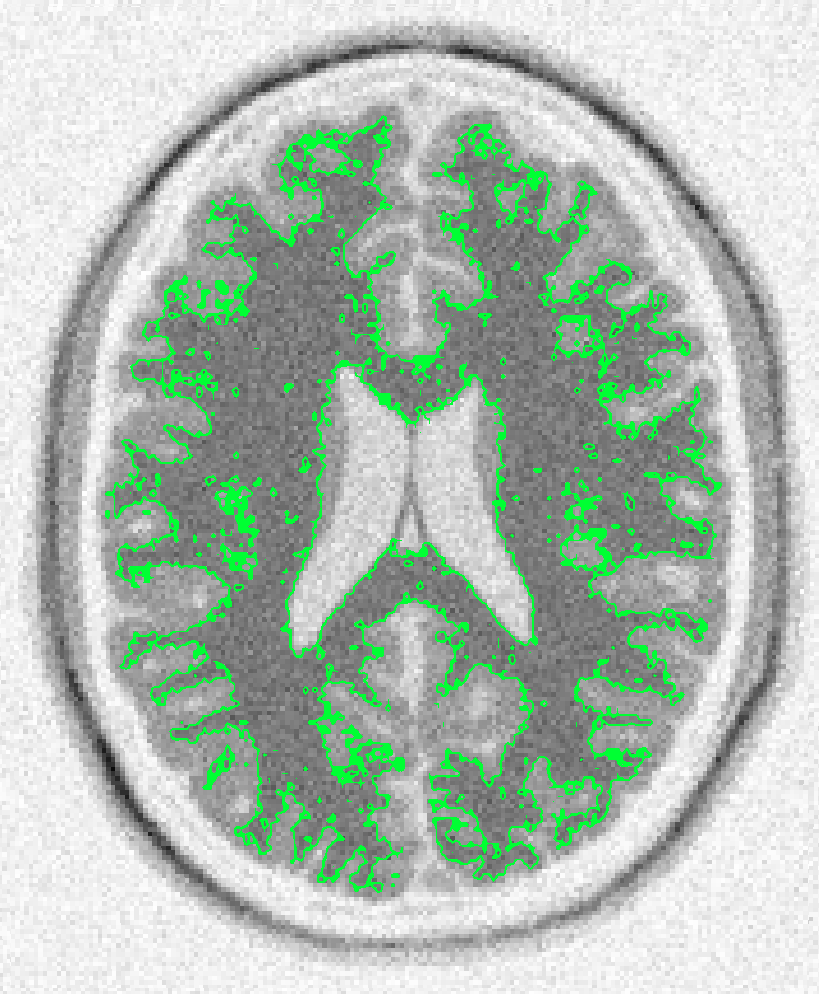
\includegraphics[width=3.05in]{figures/WithoutCurvature.png}
}
\subfigure[the same segmentation as above, using the same parameters, but under the influence of the curvature term]{
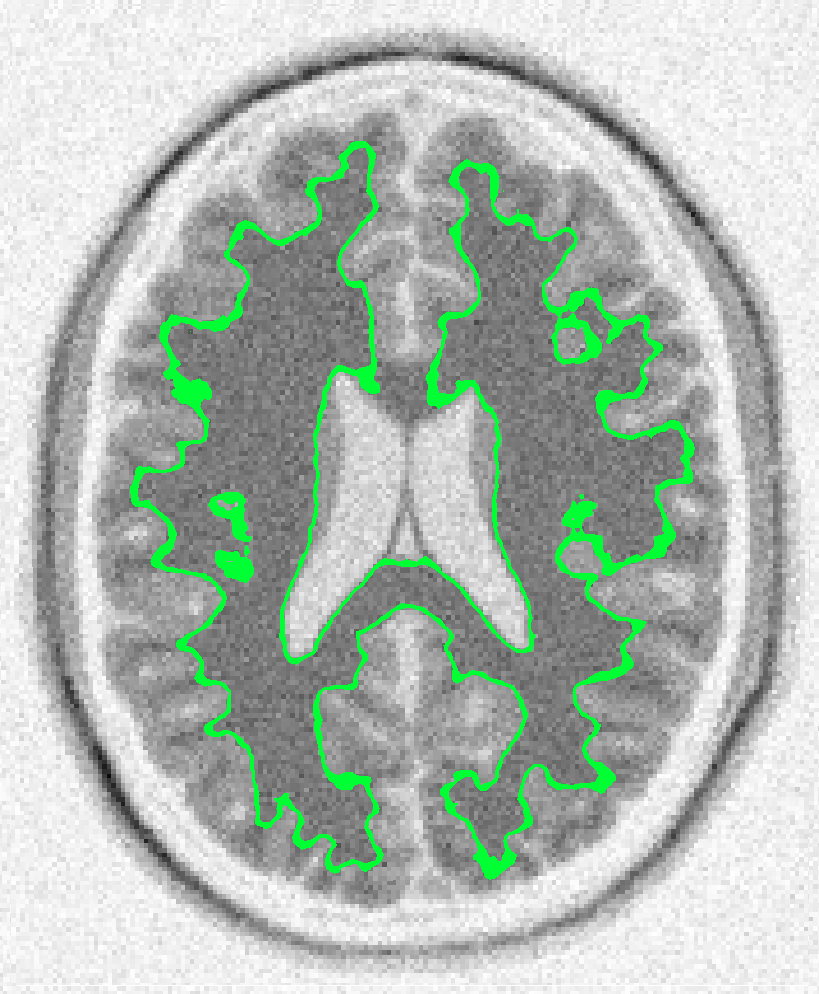
\includegraphics[width=3.05in]{figures/WithCurvature.png}
}
\caption{The effect of the curvature term in my speed function.}
\label{fig:curvatureeffect}
\end{figure}
%*******************************************************************************

As proposed by Lefohn et al.~\cite{Lefohn-2003-MICCAI,Lefohn-2003-Vis,Lefohn-2004}, I define the data term of my speed function $D \leftbracket \boldx \rightbracket = \varepsilon - \leftbracket \leftvbracket \ix \rightvbracket - T \rightbracket $ to be a function of the image intensity $\ix$, the user-specified target intensity $T$ that will encourage maximal surface growth, and a user-specified intensity window parameter $\varepsilon $ within which the level set surface is encouraged to grow. If $\ix$ is between $T-\varepsilon $ and $T+\varepsilon $, then $D \leftbracket \boldx \rightbracket $ will encourage surface growth, otherwise $D \leftbracket \boldx \rightbracket $ will encourage surface contraction. I define the curvature term of my speed function as $ C \leftbracket \boldx , t \rightbracket = \curvatureterm $, where $ \curvatureterm $ is the local mean surface curvature of the level set field from the previous iteration.

I define my speed function as $ F \leftbracket \boldx , t \rightbracket = \alpha C \leftbracket \boldx , t \rightbracket + \leftbracket 1 - \alpha \rightbracket D \leftbracket \boldx \rightbracket $ where $\alpha \in \leftsbracket 0 , 1 \rightsbracket $ is a user-specified blending term that controls the relative influence of the curvature and data terms on the behavior of my speed function. Figure \ref{fig:curvatureeffect} shows the effect of adjusting the relative influence of the curvature and data terms. For a detailed account of how this speed function can be implemented efficiently, I refer the reader to Lefohn et al.~\cite{Lefohn-2004}.

Intuitively speaking, I implicitly define my level set surface as the zero-level isosurface of a scalar field $\phi$. I implicitly evolve my level set surface by updating the scalar field $\phi$. Formally speaking, for the scalar field $ \phixt : \mathfrak{R}^4 \mapsto \mathfrak{R} $, I define my level set surface as $ \leftcbracket \boldx \mid \phixt = 0 \rightcbracket$. I express the level set field update equation as follows,
\begin{equation}
    \phixt = \phixtmdt + \Delta t F \leftbracket \boldx , t \rightbracket \leftvbracket \nabla \phixtmdt \label{eq:levelseteq}
\rightvbracket
\end{equation}
Two distinct algorithms for efficiently solving Equation~\ref{eq:levelseteq} are directly relevant to my work: the GPU narrow band algorithm~\cite{Lefohn-2003-MICCAI,Lefohn-2003-Vis,Cates-2004,Lefohn-2004,Jeong-2009} and the sparse field algorithm~\cite{Whitaker-1998,Peng-1999}.


%-------------------------------------------------------------------------
\subsection{The GPU Narrow Band Algorithm}

The narrow band algorithm~\cite{Adalsteinsson-1995} only computes level set field updates inside a small region (i.e. a narrow band) of elements around the implicitly defined level set surface. This algorithm has been successfully ported to the GPU~\cite{Lefohn-2003-MICCAI,Lefohn-2003-Vis,Cates-2004,Lefohn-2004,Jeong-2009} by using various virtual memory paging schemes to map the irregular and dynamic narrow band onto a physically contiguous domain better suited for GPU computation. These virtual memory paging schemes partition the level set field into tiles and map each active tile (i.e. each tile containing elements in the narrow band) to a contiguous physical block of GPU memory. GPU narrow band algorithms only perform level set computations on active tiles. This significantly improves performance and saves a large amount of GPU memory because inactive virtual tiles do not need to be stored on the GPU. In turn, this allows for images larger than the size of available GPU memory to be segmented.

Until very recently, GPU narrow band algorithms~\cite{Lefohn-2003-MICCAI,Lefohn-2003-Vis,Cates-2004,Lefohn-2004} have maintained the narrow band by using parallel data reduction techniques on the GPU in cooperation with the CPU. The GPU generates a down-sampled memory image of active tiles which is subsequently downloaded by the CPU at the end of each iteration. The CPU is responsible for traversing the down-sampled image, determining the narrow band for the next iteration, and communicating this result back to the GPU. Since the CPU must sequentially traverse the down-sampled image when updating the narrow band, these algorithms have $O(n)$ work-complexity~\cite{Atallah-1998} and $O(n)$ step-complexity~\cite{Nyland-2000} where $n$ is the size of the active computational domain. Moreover since the CPU work for each iteration cannot begin until the GPU work is finished and vice versa, these algorithms are limited by the communication latency between the GPU and CPU.

Developed in parallel with my own work, the GPU narrow band algorithm very recently described by Jeong et al.~\cite{Jeong-2009} avoids the communication latency inherent in previous GPU narrow band algorithms by traversing the domain of active tiles in parallel on the GPU. When a thread determines that a new tile should become part of the narrow band, the thread appends that tile to a list of active tiles stored in GPU memory. Since many threads are potentially appending to this list in parallel, Jeong et al.\ use GPU atomic memory operations to serialize access to the list. Therefore this system also has $O(n)$ work-complexity and $O(n)$ step-complexity.

%-------------------------------------------------------------------------
\subsection{The Sparse Field Algorithm}

In contrast to the GPU narrow band algorithm, the sparse field algorithm~\cite{Whitaker-1998,Peng-1999} incrementally updates a linked list of active elements on the CPU during each iteration. Therefore this algorithm's work-complexity is $O(n)$. The sparse field algorithm also reduces its total amount of work by a constant factor by tracking the active computational domain at the granularity of individual elements instead of tiles. Historically the sparse field algorithm has been poorly suited to parallel implementation due to its reliance on linked lists. Aside from the literature arising from the research in this thesis (see Appendix \ref{app:hpg}), no parallel implementation of the sparse field algorithm exists in the literature.

GPU narrow band systems~\cite{Lefohn-2003-MICCAI,Lefohn-2003-Vis,Cates-2004,Lefohn-2004,Jeong-2009} have historically outperformed optimized sequential sparse field systems~\cite{Ibanez-2005}. Nonetheless the GPU narrow band system I test in this thesis takes over 100 seconds to converge on the white and grey matter in a ${256}^3$ MRI of a human head on a state-of-the-art GPU. This limitation constrains clinical applications and motivates my work-efficient and step-efficient algorithm, which leverages ideas from both the GPU narrow band algorithm and the sparse field algorithm. I begin the presentation of my algorithm by describing my novel method for tracking the active computational domain.


\fancyhead[RO,LE]{\thepage}
\fancyfoot{} 
\chapter{Maintaining a Spatially and Temporally Coherent Active Computational Domain}
\label{chapter:temporal}

The narrow band and sparse field algorithms described in the previous chapter avoid unnecessary computation by only updating field elements near the level set surface. In this chapter I make the observation that even computations near the level set surface can be avoided in regions where the level set field has locally converged. Leveraging this insight I present an algorithm for tracking the active computational domain that is coherent in space and time.

I define the minimal set of active coordinates at time $t$ as follows:
%*******************************************************************************
\begin{equation}
    A \leftbracket t \rightbracket = \leftcbracket \boldx \in \domainphi \mid \phixt \ne \phixtmdt \rightcbracket
\label{eq:minimal}
\end{equation}
%*******************************************************************************
$A\leftbracket t \rightbracket$ is the minimal set of coordinates that must be updated at time $t$ to ensure the correctness of my algorithm because if $\phixt = \phixtmdt$, then a new value does not have to be written into the level set field at $\boldx$ and if $\phixt \neq \phixtmdt$ then I must calculate the new value $\phixt$ and write it to the level set field at $\boldx$. 

From Equation~\ref{eq:minimal} I derive two conditions, each of which is sufficient to imply that $ \boldx  \notin A \leftbracket t \rightbracket $. Both of these conditions are inexpensive to compute from local properties of the level set field and are independent of my application-specific speed function. These conditions could therefore be applied in a variety of level set simulations.

The intuition behind the first condition ${ \varsigma }_{1}$ is that computation can be avoided in regions of the level set field that are far away from the level set surface. In this sense, ${ \varsigma }_{1}$ maintains an active computational domain that is coherent in space. Formally speaking, regions that are far away from the level set surface are guaranteed to have a gradient magnitude of zero. Therefore ${ \varsigma }_{1}$ can be expressed as follows:
%*******************************************************************************
\begin{equation}
    \conditionone \equiv \leftvbracket \nabla \phixtmdt \rightvbracket = 0
\label{eq:conditionone}
\end{equation}
%*******************************************************************************
The fact that $\conditionone$ implies $\boldx \notin A\leftbracket t \rightbracket$ follows directly from  Equation~\ref{eq:levelseteq}. I note that ${ \varsigma }_{1}$ has been described previously by Lefohn et al.~\cite{Lefohn-2003-Vis,Lefohn-2004}.

The intuition behind the second condition ${ \varsigma }_{2}$ is that computation can be avoided in regions of the level set field which have locally converged, which will have a temporal derivative of zero. In this sense, ${ \varsigma }_{2}$ maintains an active computational domain that is coherent in time. I define the set $ \nx $ as the set of all coordinates in the immediate neighborhood of $ \boldx $ (including $  \boldx $ itself). I observe that if $ \phixtmdt = \phixtmtdt $, then $ \frac{ \Delta \phi \leftbracket \boldx \rightbracket }{ \Delta t } = 0 $. In other words if the level set field value is constant from one iteration to the next at $ \boldx $, then $ \phi $ is in a state of temporal equilibrium at $ \boldx $. Assuming the speed function is defined locally, the only event that could potentially disrupt this state of temporal equilibrium at $ \boldx $ is if $ \phi \leftbracket \boldn \rightbracket $ changes for some neighbor $ \boldn \in \nx $. If the level set field is in a state of temporal equilibrium in the neighborhood around $ \boldx $ at time $ t - 2 \Delta t $, then $ \boldx $ will continue to be in a state of temporal equilibrium at time $ t - \Delta t $. This leads to the following expression for ${ \varsigma }_{2}$:
%*******************************************************************************
\begin{equation}
\conditiontwo \equiv { \forall }_{ \boldn \in \nx } : \phi \leftbracket \boldn , t - \Delta t \rightbracket = \phi \leftbracket \boldn , t - 2 \Delta t \rightbracket
\label{eq:conditiontwo}
\end{equation}
%*******************************************************************************
I include a more formal derivation of ${ \varsigma }_{2}$ in Appendix~\ref{app:temporal}.
As far as I know ${ \varsigma }_2 $ is a novel contribution to the literature.

For the logical \emph{not} operator $\lnot$ I formally express the active set $A$ at time $t$ as follows:
%*******************************************************************************
\begin{equation}
A \leftbracket t \rightbracket = 
\begin{cases} 
    \domainphi                                                                                                                      & t = 0        \\
    \leftcbracket \boldx \mid \lnot \conditionone \rightcbracket                                                                    & t = \Delta t \\
    \leftcbracket \boldx \mid \lnot \conditionone \rightcbracket \cap \leftcbracket \boldx \mid \lnot \conditiontwo \rightcbracket  & t > \Delta t \\
\end{cases}
\label{eq:active}
\end{equation}
%*******************************************************************************

%*******************************************************************************
% Algorithmic Overview
\begin{figure*}[t]
\centering
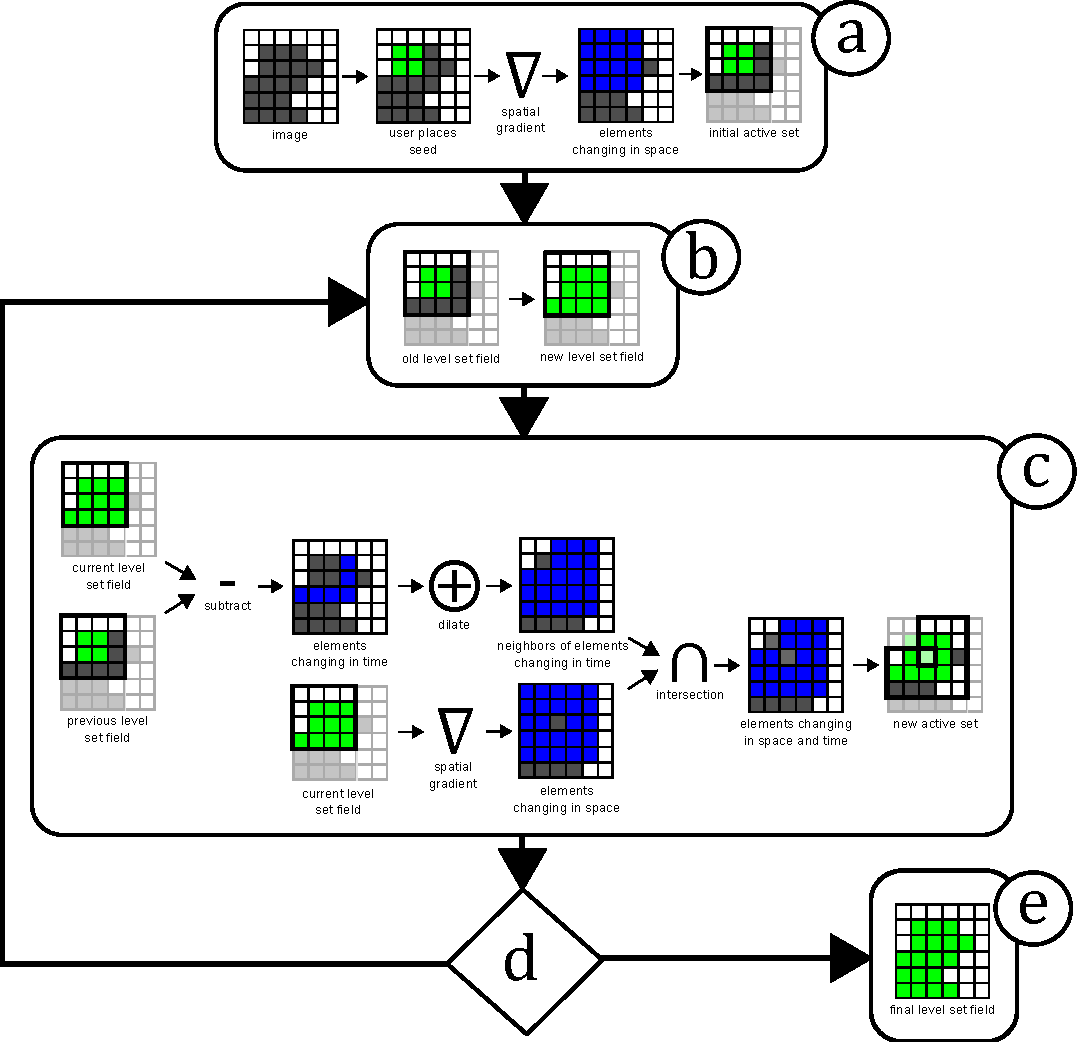
\includegraphics[width=6.0in]{figures/Algorithm.pdf}
\caption{My algorithm for tracking the active computational domain. Image data is shown in grey, currently segmented regions are shown in green, and intermediate results for computing the active computational domain are shown in blue. The active computational domain is outlined in black, and inactive elements are shown as partially transparent. The user places a seed to initialize the level set field and the initial active computational domain is determined according to the spatial derivatives of the level set field (a). During each iteration the level set field is updated at all active elements (b). The new active computational domain is computed according to the temporal and spatial derivatives of the level set field (c). If the new active computational domain is empty (d) then the segmentation has globally converged (e). Otherwise I go to (b). }
\label{fig:algorithm}
\end{figure*}
%*******************************************************************************

A diagram describing my method of tracking the active computational domain is shown in Figure~\ref{fig:algorithm} and sequential psuedo-code for this algorithm is given in Listing \ref{alg:levelset-sequential-init} and Listing \ref{alg:levelset-sequential-update}. During initialization, my algorithm initializes the level set field and then computes the initial active set according to ${\varsigma}_{1}$ only (Figure \ref{fig:algorithm}a). This is because  ${ \varsigma }_{2}$ looks for regions of the level set field that have converged with respect to time, and during initialization there are no such regions. In other words ${\varsigma}_{2}$ relies on backward time derivatives of the level set field which are initially undefined. During each iteration, my algorithm performs the level set field update on all active voxels according to Equation \ref{eq:levelseteq} (Figure \ref{fig:algorithm}b). After updating $ \phi$, the set of active voxels must itself be updated. The algorithm must then remove any voxels that are no longer active and add all voxels that have become active to the active set. Since either ${\varsigma}_1 $ or ${\varsigma}_2 $ is sufficient to exclude a voxel from the active set, both ${\varsigma}_1 $ and ${\varsigma}_2 $ must be false for the corresponding voxel to be included in the active set (Figure \ref{fig:algorithm}c). If the updated active set is empty (Figure \ref{fig:algorithm}d) then the segmentation has converged (Figure \ref{fig:algorithm}e).
During each iteration, this algorithm performs work proportional only to the size of the active computational domain. The work performed during each iteration is independent of the size of the level set field

%*******************************************************************************
\begin{Listing}[]
    \caption{Sequential pseudo code for initializing the level set field and active computational domain. The level set field is initialized to the signed and clamped distance transform relative to a user-specified seed sphere with the center \textbf{c} and the radius \textit{r}. The initial active computational domain is determined according to the spatial derivatives of the level set field on line 9.}
    \begin{algorithmic}[1]
        \FORALL { coordinates $ \boldx \in \domainphi $ } 
            \STATE { $ \phi \leftbracket \boldx , 0 \rightbracket \gets \mbox{clamp} \leftbracket \| \boldx - \mathbf{c} \|- r \rightbracket $ }
        \ENDFOR
        \STATE { $ A\leftbracket \Delta t \rightbracket \gets \emptyset $ }        
        \FORALL { coordinates $ \boldx \in \domainphi $ } 
            \STATE { $ g \gets \mbox{false} $ }
            \FORALL { coordinates $ \boldn \in \nx $ }
                \IF { $\mbox{\textbf{not }} g $ }
                    \IF { $ \phi \leftbracket \boldx , 0 \rightbracket \neq \phi \leftbracket \boldn , 0 \rightbracket $ }
                        \STATE { $ g \gets \mbox{true} $ }
                    \ENDIF
                \ENDIF
            \ENDFOR
            \IF { $ g $ }   
                \STATE { $ A \leftbracket \Delta t \rightbracket \gets A \leftbracket \Delta t \rightbracket \cup \leftcbracket \boldx \rightcbracket $ }
            \ENDIF
        \ENDFOR
    \end{algorithmic}
    \label{alg:levelset-sequential-init}
\end{Listing}
%*******************************************************************************

%*******************************************************************************
\begin{Listing}[t]
    \caption{Sequential pseudo code for updating the level set field and active computational domain until the segmentation has converged. The active computational domain is determined according to the spatial and temporal derivatives of the level set field on line 10.}
    \begin{algorithmic}[1]
        \STATE { $ t \gets \Delta t $ }
        \WHILE { $ A\leftbracket t \rightbracket \neq \emptyset $ }
            \FORALL { coordinates $\boldx \in A\leftbracket t \rightbracket $ }
                \STATE { $ \phixt \gets \phixtmdt + \Delta t F\leftbracket \boldx , t \rightbracket \leftvbracket \nabla \phixtmdt \rightvbracket $ }
            \ENDFOR
            \STATE { $ A\leftbracket t + \Delta t \rightbracket \gets \emptyset $ }            
            \FORALL { coordinates $\boldx \in A\leftbracket t \rightbracket $ }
                \STATE { $g \gets \mbox{false}$ }
                \FORALL { coordinates $\boldn \in \nx$ }
                    \IF { $ \phixt \neq \phi \leftbracket \boldn , t \rightbracket \mbox{\textbf{ and }} \phixt \neq \phixtmdt $ }
                        \STATE { $ g \gets \mbox{true} $ }
                        \STATE { $ A\leftbracket t + \Delta t \rightbracket \gets A\leftbracket t + \Delta t \rightbracket \cup \leftcbracket \boldn \rightcbracket $ }      
                    \ENDIF
                \ENDFOR
                \IF { $ g $ }   
                    \STATE { $ A\leftbracket t + \Delta t \rightbracket \gets A\leftbracket t + \Delta t \rightbracket \cup \leftcbracket \boldx \rightcbracket $ }      
                \ENDIF
            \ENDFOR
            \STATE { $ t \gets t + \Delta t $ }
        \ENDWHILE
    \end{algorithmic}
    \label{alg:levelset-sequential-update}    
\end{Listing}
%*******************************************************************************


\fancyhead[RO,LE]{\thepage}
\fancyfoot{} 
\chapter{An Efficient Parallel Algorithm}
\label{chapter:parallel}

In the previous chapter, I describe a sequential algorithm for updating the level set field according to a sparse and dynamic active computational domain that is coherent in space and time. In this chapter I map this sequential algorithm onto massively parallel hardware.

Parallelizing the sequential algorithm from the previous chapter is challenging because the algorithm assumes the availability of mathematical sets (i.e. collections that are guaranteed not to contain duplicate elements) in the progamming model. The following scenario highlights the difficulty of implementing the functionality of mathematical sets on massively parallel hardware. Suppose two threads want to simultaneously add the same element to a set. Suppose this element does not currently exist in the set. Without proper synchronization, it will appear to both threads as though the element does not exist in the set. In this case both threads will decide that they must add the same element to the set. After both threads add the same element to the set, the element will then appear in the set twice. Therefore the set will fail to exclude duplicate elements. Solving this problem with per-thread synchronization mechanisms like locks and atomic memory operations scales poorly on massively parallel hardware.

\section{Algorithm Overview}

For reasons described in Chapter \ref{chapter:background}, I prefer parallel algorithms that are both work-efficient and step-efficient. Since the sequential algorithm in the previous chapter has $O(n)$ work-complexity, I would prefer the parallelized version of this algorithm to have work-complexity of at most $O(n)$ and step-complexity of at most $O(\log n)$. This upper bound on work-complexity and step-complexity motivates the parallel algorithm described in this chapter.

\begin{samepage}
A high level overview of my parallel algorithm is as follows:

\begin{enumerate}

    \item Initialize the level set field and generate a dense list of active coordinates.

    \item Update the level set field at all active coordinates.

    \item Generate new active coordinates. During this step generating duplicate active coordinates is permitted.

    \item Remove all duplicate active coordinates generated in (3).

    \item Compact all the unique new active coordinates from (4) into a new dense list.

    \item If there are no active coordinates in the new dense list, the segmentation has globally converged. Otherwise go to (2).

\end{enumerate}
\end{samepage}

%-------------------------------------------------------------------------
\section{Assumptions}
\label{subsec:assumptions}

I assume $ \phi $ is 3D and the voxels in $ \phi $ are 6-connected. Therefore it is guaranteed that for all voxels $ \boldx \in \domainphi $, the set $ \nx $ contains at most seven elements: the 6-connected neighbors of $ \boldx $ and $ \boldx $ itself. I define the set $ E = \leftcbracket \leftbracket 0,0,0 \rightbracket , \leftbracket \pm 1,0,0 \rightbracket , \leftbracket 0,\pm 1,0 \rightbracket , \leftbracket 0,0,\pm 1 \rightbracket \rightcbracket $ as the set of offset vectors from a voxel to its 6-connected neighbors.

%-------------------------------------------------------------------------
\section{Data Structures and Notation}
\label{subsec:dataStructuresAndNotation}

My algorithm requires three 3D buffers: $\phiwrite$ and $\phiread$ to store the current and previous level set field respectively; and $U$ to use as a scratchpad. My algorithm also requires eight 1D buffers: $V$ to store the current dense list of active coordinates; and $B^{ \leftbracket 0,0,0 \rightbracket }$, $B^{ \leftbracket \pm 1,0,0 \rightbracket }$, $B^{ \leftbracket 0, \pm 1,0 \rightbracket }$, and $B^{ \leftbracket 0,0, \pm 1 \rightbracket }$ to use as auxiliary buffers when generating new active coordinates. The size of each buffer is equal to the size of the entire level set field. All buffers are initially filled with null values.

I use a subscript notation to refer to individual buffer elements. For example $V_i$ refers to the $i^{th}$ element of $V$; $V_{j \ldots k }$ refers to the range of elements in $V$ from $V_j$ to $V_k$; and $U_{\boldx}$ refers to the element of $U$ with the 3D coordinates $\boldx$.

%We use $V$ to store the current set of active coordinates. We use $\phiread$ and $\phiwrite$ to read from and write to the level set field in a double-buffered fashion. We use $ B^{ \leftbracket 0,0,0 \rightbracket }$, $B^{ \leftbracket 0,0, \pm 1 \rightbracket }$, $B^{ \leftbracket 0, \pm 1,0 \rightbracket }$, and $B^{ \leftbracket \pm 1,0,0 \rightbracket }$ as auxiliary buffers to store intermediate output as we're generating new active coordinates. Finally we use $U$ as a scratchpad buffer. All buffers are initially filled with null values.

%-------------------------------------------------------------------------
\section{Initialization}
\label{subsec:initialization}


\begin{Listing}[t]
    \caption{Initializing the level set field to the signed and clamped distance transform relative to a user-specified seed sphere with the center \textbf{c} and the radius \textit{r}. \label{pseudo:1} }
    \begin{algorithmic}[1]
        \FORALL { coordinates $\boldx \in \domainphi$ in parallel } 
            \STATE { $ \phiread_{\boldx} \gets \mbox{clamp} \leftbracket \| \boldx - \mathbf{c} \| - r \rightbracket $  }
            \STATE { $ \phiwrite_{\boldx} \gets \mbox{clamp} \leftbracket \| \boldx - \mathbf{c} \| - r \rightbracket $  }
        \ENDFOR
    \end{algorithmic}
\end{Listing}


\begin{Listing}[t]
    \caption{Initializing the list of active coordinates. The spatial derivative of the level set field is tested on line 5. \label{pseudo:2} }
    \begin{algorithmic}[1]
        \FORALL { coordinates $\boldx \in \domainphi$ in parallel }
            \STATE { $ g \gets \mbox{false} $ }
            \FORALL { coordinates $\boldn \in \nx$ }
                \IF { \textbf{not } $ g $ }
                    \IF { $ \phiread_{\boldx} \neq \phiread_{\boldn} $  }
                        \STATE { $ g \gets \mbox{true} $ }
                    \ENDIF    
                \ENDIF
            \ENDFOR
            \IF { $ g $ }
                \STATE { $ U_{\boldx} \gets \boldx $  }
            \ENDIF           
        \ENDFOR
        \STATE { $ V \gets \mbox{\textbf{compact}} \leftbracket U \rightbracket $  }
    \end{algorithmic}
\end{Listing}


I initialize in parallel every coordinate in $\phiread$ and $\phiwrite$ according to a user-specified seed region as shown in Listing~\ref{pseudo:1}. For more details on this initialization step I refer the reader to Lefohn et al.~\cite{Lefohn-2004}.

I then generate a densely packed buffer of active coordinates $V$ based on the contents of $\phiread$ as shown in Listing~\ref{pseudo:2}. I test every coordinate of $\phiread$ in parallel to determine which ones are active. If a coordinate is deemed active according to Equation~\ref{eq:active}, I write that coordinate to my 3D scratchpad $U$ using the coordinate itself as the 3D array index. I compact $U$ in parallel to produce $V$. I set the initial size of the active computational domain $n$ to be the number of coordinates that were compacted into $V$. I note that since $U$ contains either a unique value or null at all coordinates, it is guaranteed that there are no duplicate coordinates in $V_{0 \ldots n}$. At this point my algorithm has been fully initialized. I avoid traversing the entire level set field for the remainder of my algorithm.


%*******************************************************************************
% FIGURE 2
%\begin{figure}[t]
%\centering
%\includegraphics[width=6.0in]{figs/fig2.png}
%\caption{Initializing our list of active coordinates in parallel. We initialize in parallel a scratchpad buffer with active coordinates using the coordinates themselves as array indices. We then interpret the scratchpad buffer as one-dimensional and compact it in parallel to produce a densely packed buffer of active coordinates.}
%\label{fig:2}
%\end{figure}
%*******************************************************************************


%-------------------------------------------------------------------------
\section{Updating the Level Set Field}
\label{subsec:updatingTheLevelSetField}


\begin{Listing}[t]
    \caption{Updating the level set field according to Equation~\ref{eq:levelseteq} and clearing the scratchpad at all active coordinates. $n$ is the current size of the active computational domain. \label{pseudo:3} }
    \begin{algorithmic}[1]
        \FORALL { coordinates $\boldv \in V_{0 \ldots n}$ in parallel }
            \STATE { $ \phiwrite_{\boldv} \gets \phiread_{\boldv} + \Delta t F \leftbracket \boldv , t \rightbracket \ \leftvbracket \nabla \phiread_{\boldv} \rightvbracket $ }        
            \STATE { $ U_{\boldv} \gets \mbox{null} $  }                
        \ENDFOR
        \STATE { $ \mbox{\textbf{swap}} \leftbracket \phiread, \phiwrite \rightbracket $  }        
    \end{algorithmic}
\end{Listing}



During each iteration I update $\phiwrite$ and clear $U$ at all active coordinates as shown in Listing~\ref{pseudo:3}. This is guaranteed to completely clear $U$ because the only non-null values in $U$ are at active coordinates, each of which was previously compacted into $V$. At this point I am finished updating the level set field for this iteration, so I swap references to $\phiread$ and $\phiwrite$.

It is important to note that for a given iteration $t$, it is actually the case that $\phiwrite = \phi \leftbracket t - 2 \Delta t \rightbracket $ and $ \phiread = \phi \leftbracket t - \Delta t \rightbracket $ prior to writing new level set values into $\phiwrite$. Since I do not update every voxel at every iteration, I must ensure that the old values from $t - 2 \Delta t$ are allowed to remain in $ \phiwrite $ only if they have not changed from iteration $t - 2 \Delta t$ to iteration $t - \Delta t$. Otherwise I must ensure that these values are updated. Fortunately if $\phixtmtdt \neq \phixtmdt $, then Equation \ref{eq:active} guarantees $ \boldx \in A \leftbracket t \rightbracket $ and a new level set value that depends only on $ \phiread = \phi \leftbracket t - \Delta t \rightbracket $ will be written into $ \phiwrite $ at $ \boldx $.



%-------------------------------------------------------------------------
\section{Generating New Active Coordinates}
\label{subsec:generatingNewActiveCoordinates}


%*******************************************************************************
% FIGURE 3
\begin{figure}[t]
\centering
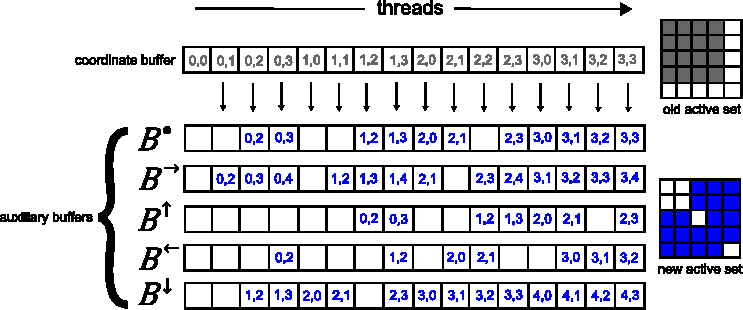
\includegraphics[width=6.0in]{figures/NewActive.pdf}
\caption{Generating new active coordinates. There may be duplicate coordinates in the auxiliary buffers when taken collectively. All duplicate coordinates must subsequently be removed (see Figure~\ref{fig:4}).}
\label{fig:3}
\end{figure}
%*******************************************************************************


%*******************************************************************************
\begin{Listing}[t]
    \caption{Generating new active coordinates. The temporal and spatial derivatives of the level set field are tested on line 5. $n$ is the current size of the active computational domain. \label{pseudo:4} }
    \begin{algorithmic}[1]
        \FOR { $h \gets 0$ to $n$ in parallel }
            \STATE { $\boldv \gets V_h$ } 
            \STATE { $g \gets \mbox{false}$ }
            \FORALL { coordinates $\boldn \in \nv$ }
                \IF { $ \phiread_{\boldn} \neq \phiwrite_{\boldn} $ \textbf{ and } $ \phiread_{\boldn} \neq \phiread_{\boldv} $ }
                    \STATE { $g \gets \mbox{true}$ }
                    \STATE { $\mathbf{e} \gets \boldn - \boldv$ }
                    \STATE { $B^{\mathbf{e}}_{h} \gets \boldn $ }
                \ENDIF
            \ENDFOR
            \IF { $g$ }
                \STATE { $B^{ \leftbracket 0,0,0 \rightbracket }_{h} \gets \boldv $ }
            \ENDIF                    
        \ENDFOR
    \end{algorithmic}
\end{Listing}
%*******************************************************************************


I traverse my current list of active coordinates in parallel and test for new active coordinates according to Equation~\ref{eq:active}. I describe this process in Listing~\ref{pseudo:4} and Figure~\ref{fig:3}. I test $ { \varsigma }_{1} $ and $ { \varsigma }_{2} $ for the next iteration by examining $ \phiread = \phi \leftbracket t \rightbracket $ and $ \phiwrite = \phi \leftbracket t - \Delta t \rightbracket$. I note that at the end of this step, the seven auxiliary buffers may contain duplicate coordinates when taken collectively. This is because each thread tests a local neighborhood of coordinates and some coordinates may be tested repeatedly by different threads. For example some thread $p$ may deem a coordinate $\mathbf{r}$ to be active. For the thread $p$ suppose that $\mathbf{r}-\mathbf{v}_p = \leftbracket 0,0,1 \rightbracket$ and therefore thread $p$ writes $\mathbf{r}$ to the auxiliary buffer $B^{ \leftbracket 0,0,1 \rightbracket }$. Some different thread $q$ may also deem the same coordinate $\mathbf{r}$ to be active. For the thread $q$ suppose that $\mathbf{r} - \mathbf{v}_q = \leftbracket 1,0,0 \rightbracket $ and therefore thread $q$ writes $\mathbf{r}$ to the auxiliary buffer $B^{ \leftbracket 1,0,0 \rightbracket }$. In this case $\mathbf{r}$ appears in both $B^{ \leftbracket 0,0,1 \rightbracket }$ and $B^{ \leftbracket 1,0,0 \rightbracket }$.


I also note that since each new active coordinate is the 6-connected neighbor of some old active coordinate, and all 6-connected neighbors of all old active coordinates are tested by at least one thread, it is guaranteed that all new active coordinates are contained in at least one of the seven auxiliary buffers.


%-------------------------------------------------------------------------
\section{Removing Duplicate Active Coordinates}
\label{subsec:removingDuplicateActiveCoordinates}


%*******************************************************************************
% FIGURE 4
\begin{figure}[t]
\centering
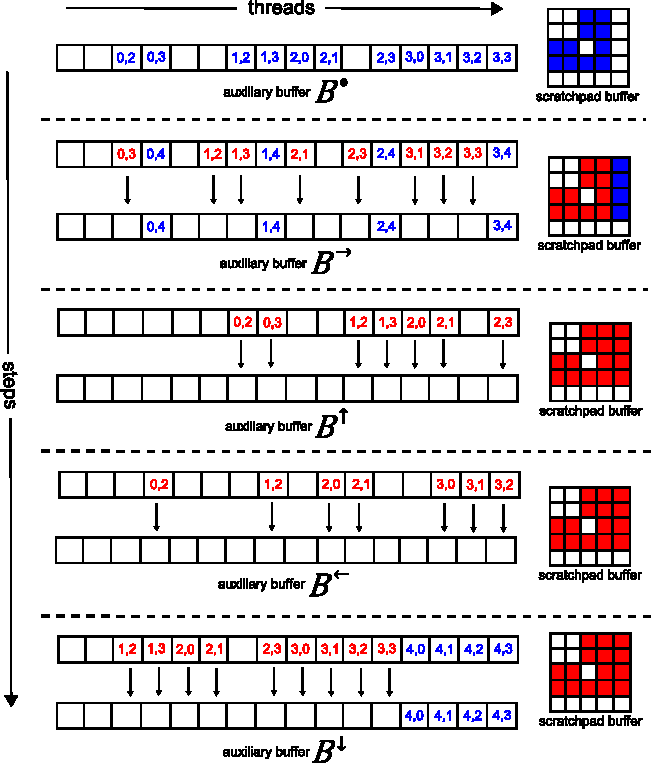
\includegraphics[width=6.0in]{figures/RemoveDuplicates-Alt.pdf}
\caption{Removing duplicate coordinates from the auxiliary buffers in parallel without sorting. Coordinates that have not been previously tagged in the scratchpad buffer are shown in blue. Coordinates that have been previously tagged in the scratchpad buffer are shown in red, and are removed from their containing auxiliary buffer. This process is free of race conditions because each step examines one auxiliary buffer and there are no duplicate coordinates within each auxiliary buffer.}
\label{fig:4}
\end{figure}
%*******************************************************************************

%*******************************************************************************
\begin{Listing}[t]
    \caption{Generating a new dense list of unique active coordinates without sorting the auxiliary buffers. $n$ is the current size of the active computational domain. \label{pseudo:5} }
    \begin{algorithmic}[1]
        \STATE { $ E' \gets E - \leftcbracket \leftbracket 0,0,0 \rightbracket , \leftbracket 0,0,1 \rightbracket \rightcbracket $ }
        \FORALL { coordinates $\mathbf{b} \in B^{ \leftbracket 0,0,0 \rightbracket }_{0 \ldots n}$ in parallel }
            \IF { $ \mathbf{b} \neq \mbox{null}$ }
                \STATE { $ U_{\mathbf{b}} \gets \mbox{tagged}$ }
            \ENDIF
        \ENDFOR                        
        \FORALL { offset vectors $\mathbf{e} \in E' $ } 
            \FOR { $h \gets 0$ to $n$ in parallel }
                \STATE { $\mathbf{b} \gets B^{\mathbf{e}}_{h}$ }            
                \IF { $ \mathbf{b} \neq \mbox{null}$ }
                    \IF { $ U_{\mathbf{b}} = \mbox{tagged} $ }
                        \STATE { $B^{\mathbf{e}}_{h} \gets \mbox{null}$ }
                    \ELSE
                        \STATE { $U_{\mathbf{b}} \gets \mbox{tagged} $ }
                    \ENDIF                                            
                \ENDIF
            \ENDFOR
        \ENDFOR
        \FOR { $h \gets 0$ to $n$ in parallel }
            \STATE { $\mathbf{b} \gets B^{ \leftbracket 0,0,1 \rightbracket }_{h} $ }       
            \IF { $ \mathbf{b} \neq \mbox{null}$ \textbf{ and } $ U_{\mathbf{b}} = \mbox{tagged} $ }
                \STATE { $B^{ \leftbracket 0,0,1 \rightbracket }_{h} \gets \mbox{null}$ }
            \ENDIF
        \ENDFOR                        
        \STATE { $V \gets \mbox{\textbf{compact}} \leftbracket
            B^{ \leftbracket 0,0,0 \rightbracket }_{0 \ldots n},
            B^{ \leftbracket \pm 1, 0, 0 \rightbracket }_{0 \ldots n},
            B^{ \leftbracket 0, \pm 1, 0 \rightbracket }_{0 \ldots n},
            B^{ \leftbracket 0, 0, \pm 1 \rightbracket }_{0 \ldots n} \rightbracket$ }       
    \end{algorithmic}
\end{Listing}
%*******************************************************************************


I make the observation that although there may be duplicate coordinates in the seven auxiliary buffers taken collectively, it is guaranteed that there are no duplicate coordinates in each of the seven auxiliary buffers taken individually. This is because there are no duplicate coordinates in $V_{0 \ldots n}$ and for all offset vectors $\mathbf{e} \in E$, either $B^{\mathbf{e}}_{i} = V_i + \mathbf{e} $ or ${B^{\mathbf{e}}_i} = \mbox{null}$ for all array indices $i$ where $0 \leq i \leq n$.

Based on the guarantee in the previous paragraph, I am able to remove all duplicate coordinates in seven passes without requiring any additional sorting or synchronization primitives. I describe this process in Listing~\ref{pseudo:5} and Figure~\ref{fig:4}.


%-------------------------------------------------------------------------
\section{Compacting the New Active Coordinates}
\label{subsec:compactingTheNewActiveCoordinates} 

I compact the seven auxiliary buffers in parallel to produce a new dense list of active coordinates and store the result in $V$ as shown in Listing~\ref{pseudo:5}. Since I only ever write to the first $n$ elements of each auxiliary buffer, I only need to compact $7n$ elements in total, rather than compacting the total size of each buffer. In order to further improve the efficiency of this buffer compacting step, I allocate the auxiliary buffers dynamically at the beginning of each iteration by partitioning a larger pre-allocated buffer.

After compacting the seven auxiliary buffers, I check if any new active coordinates were compacted into $V$. If so, I clear $B^{\mathbf{e}}_{0 \ldots n}$ for all offset vectors $\mathbf{e} \in E$, update $n$ to be the number of new active coordinates that were compacted into $V$, and go to the step described in section~\ref{subsec:updatingTheLevelSetField}. Otherwise my algorithm has globally converged on the segmented region contained in $\phiread$.


%-------------------------------------------------------------------------
\section{Improving Practical Memory Efficiency}
\label{subsec:improvingPracticalMemoryEfficiency}

All memory accesses to the 1D buffers $V$, $B^{ \leftbracket 0,0,0 \rightbracket }$, $B^{ \leftbracket \pm 1, 0, 0 \rightbracket }$, $B^{ \leftbracket 0, \pm 1, 0 \rightbracket }$, and $B^{ \leftbracket 0, 0, \pm 1 \rightbracket }$ achieve maximum efficiency on modern GPU architectures, since these memory accesses can be fully \emph{coalesced} by the hardware-managed memory controller into a small number of memory transactions. This is because the 1D buffers are always accessed via a unique thread index such that neighboring threads always access neighboring locations in memory.

In general none of the memory accesses to the 3D buffers $\phiread$, $\phiwrite$, and $U$ can be coalesced. After initialization these buffers are always accessed at sparse active coordinates which are not guaranteed to be neighboring for neighboring threads. Therefore it is not clear how my algorithm can advantage of the on-chip software-managed cache available on modern GPUs. For this reason my implementation does not use this on-chip software-managed cache.

%*******************************************************************************
% FIGURE swizzled
\begin{figure}[t]
\centering
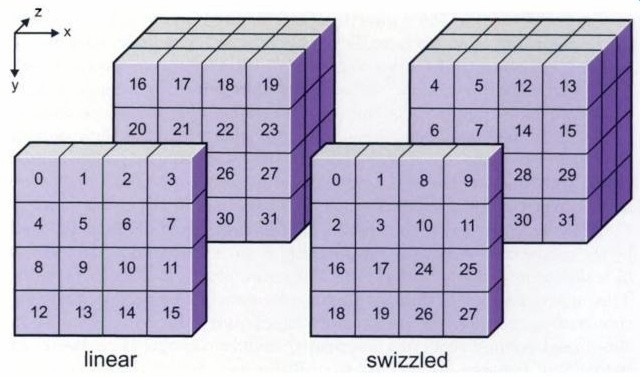
\includegraphics[width=6.0in]{figures/swizzled.jpg}
\caption{A linear memory layout with poor multi-dimensional cache locality and a swizzled memory layout that improves multi-dimensional cache locality. The blocks represent elements in a 3D array, and the numbers in each block represent the 1D location of the element in memory. The swizzled memory layout is such that elements that are nearby in 3D are more likely to be nearby in memory.~\cite{Engel-2006}}
\label{fig:swizzled}
\end{figure}
%*******************************************************************************

However since there is some spatial locality in the active computational domain, it is probable but not guaranteed that nearby active coordinates in $V$ are nearby in 3D space. I leverage this spatial locality by reading from the 3D buffers via the hardware-managed GPU texture cache. To improve multi-dimensional cache coherence, I use a simple swizzled memory layout as described by Engel et al.~\cite{Engel-2006} and shown in Figure \ref{fig:swizzled}.

In my implementation the data type of $\phiwrite$ and $\phiread$ is 32-bit floating point and the data type of all other buffers is 32-bit integer. To maximize memory efficiency when storing 3D level set field coordinates in these integer buffers, I pack the $x$, $y$, and $z$ components of each 3D coordinate into 11, 11, and 10 bits respectively. However if the level set field contains more than $2048 \times 2048 \times 1024 = 2^{32}$ elements, the data type of each integer buffer must be expanded such that the largest possible level set field coordinate can fit into a single element.


\fancyhead[RO,LE]{\thepage}
\fancyfoot{} 
\chapter{Evaluation}
\label{chapter:evaluation}

In the previous chapter I presented a massively parallel GPU algorithm for level set segmentation. In this chapter I describe a methodology for evaluating this algorithm. I analyze the asymptotic performance and memory efficiency of my algorithm. I also describe a series of experiments that compare the computational efficiency and accuracy of my GPU algorithm to the previous state-of-the-art GPU algorithm.
The results of these experiments show that my algorithm significantly outperforms previous state-of-the-art algorithms with no reduction in segmentation accuracy.%-------------------------------------------------------------------------
\section{Asymptotic Complexity}
\label{subsec:asymptoticComplexity}

The algorithm I use for buffer compacting has $O(w)$ work-complexity and $O({\log }_{2}w)$ step-complexity where $w$ is the size of the input~\cite{Sengupta-2011}. Therefore my algorithm has $O(p)$ work-complexity and $ O \leftbracket { \log }_2 p \rightbracket $ step-complexity during initialization where $p$ is the size of the entire level set field. After initialization my algorithm has $O(n)$ work-complexity and $ O \leftbracket { \log }_2 n \rightbracket $ step-complexity where $n$ is the size of the active computational domain. From this I conclude that my algorithm is both work-efficient and step-efficient. For a more detailed proof I refer the reader to Appendix~\ref{app:proof}.

My algorithm requires $O(p)$ memory. In other words the memory requirements of my algorithm increase linearly with the size of the level set field rather than the (much smaller) surface area of the segmented surface, as is the case with previous GPU algorithms~\cite{Lefohn-2003-MICCAI,Lefohn-2003-Vis,Cates-2004,Lefohn-2004,Jeong-2009}.

%-------------------------------------------------------------------------
\section{Experimental Methodology}
\label{subsec:experimentalMethodology}


I performed all my experiments on an Intel 2.5 gigahertz Xeon Processor with 4 gigabytes of memory and an NVIDIA GTX 280 GPU. I implemented my algorithm using CUDA~\cite{NVIDIACUDA-2010} and I used the open-source CUDA Data Parallel Primitives Library~\cite{CUDPP-2010} for buffer compacting. I implemented the GPU narrow band algorithm using OpenGL~\cite{Shreiner-2005} and GLSL~\cite{Rost-2006} with a tile size of $16^2$, as described by Lefohn et al.~\cite{Lefohn-2003-MICCAI,Lefohn-2003-Vis,Lefohn-2004}. I feel this is the fairest method of evaluating each algorithm since the GPU narrow band algorithm relies on hardware features not exposed in CUDA (e.g. direct write access to texture memory). Likewise my algorithm makes use of hardware features not exposed in OpenGL and GLSL (e.g. random write access to global memory).

I performed various segmentation tasks on volumetric images generated from the BrainWeb Simulated Brain Database~\cite{BrainWeb-2010,Kwan-1996,Cocosco-1997,Collins-1998,Kwan-1999}. This database can be used to generate simulated head MRIs with a variety of realistic noise characteristics in a controlled setting where the ground truth classification of each voxel is known. I repeated these segmentation tasks using my algorithm, the GPU narrow band algorithm, and a level set solver implemented in CUDA that unconditionally updates the entire level set field. I also performed various segmentation tasks on a $256 \times 256 \times 272$ abdominal CT image and a $288 \times 352 \times 112$ wrist CT image using my algorithm.

To evaluate the accuracy and variability of my algorithm, I performed a series of repeated ($N=10$) white matter segmentations on ${256}^3$ head MRIs with varying signal-to-noise ratio (SNR) values. I segmented these images using a randomly selected seed location. I measured the accuracy of each segmentation by computing the Dice Coefficient~\cite{Shattuck-2009,Jeong-2009} and the Total Correct Fraction~\cite{Lefohn-2003-MICCAI,Cates-2004}.

To evaluate the speed of my algorithm, I segmented the white and grey matter in a ${256}^3$ head MRI with $SNR=11$. I measured the computation time per iteration per subroutine and the total computation time for the segmentation. I also measured the number of active voxels per iteration and the total number of processed voxels. To provide additional context for these experiments, I repeated the segmentation task using the open-source Insight Segmentation and Registration Toolkit~\cite{Ibanez-2005}, which implements the sparse field algorithm~\cite{Whitaker-1998,Peng-1999} in single-threaded C++.

\section{Results and Discussion}

%*******************************************************************************
% FIGURE Aorta
\begin{figure}[t]
\centering
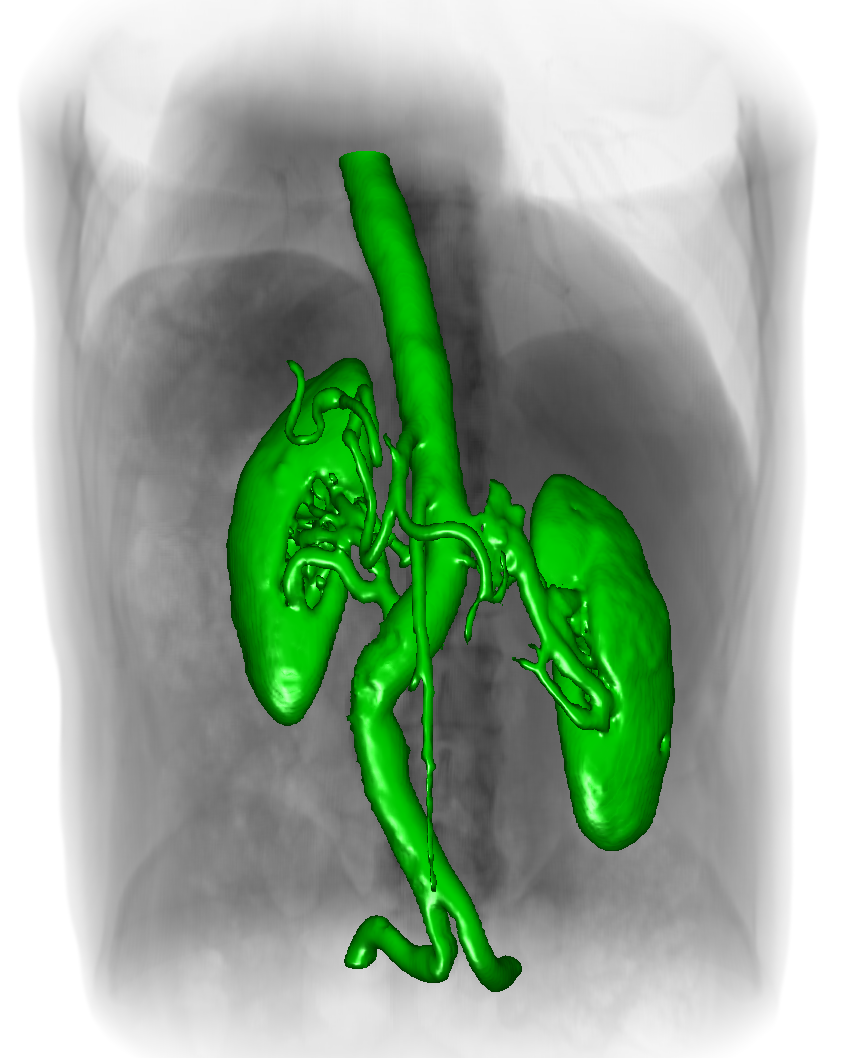
\includegraphics[width=6.0in]{figures/Aorta-3D.png}
\caption{The aorta and kidneys in a $256 \times 256 \times 272$ abdominal CT image segmented with my algorithm. The total computation time required to produce this segmentation was 16 seconds.}
\label{fig:aorta}
\end{figure}
%*******************************************************************************

%*******************************************************************************
% FIGURE Bone
\begin{figure}[t]
\centering
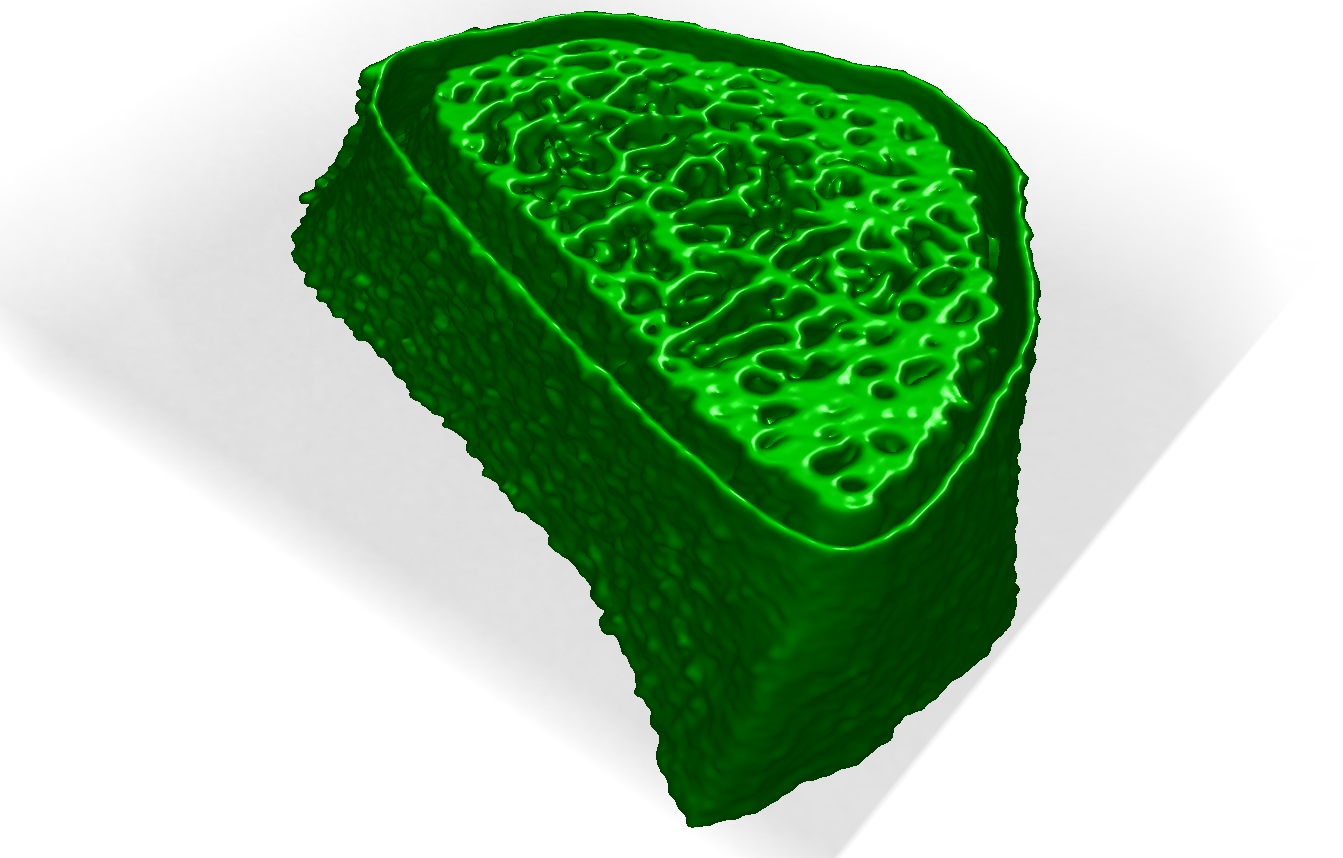
\includegraphics[width=6.0in]{figures/Bone-3D.png}
\caption{The cortical bone and trabecular bone in a $288 \times 352 \times 112$ wrist CT image segmented with my algorithm. The total computation time required to produce this segmentation was 12 seconds.}
\label{fig:bone}
\end{figure}
%*******************************************************************************

%*******************************************************************************
% FIGURE BrainWeb 3D
\begin{figure}[t]
\centering
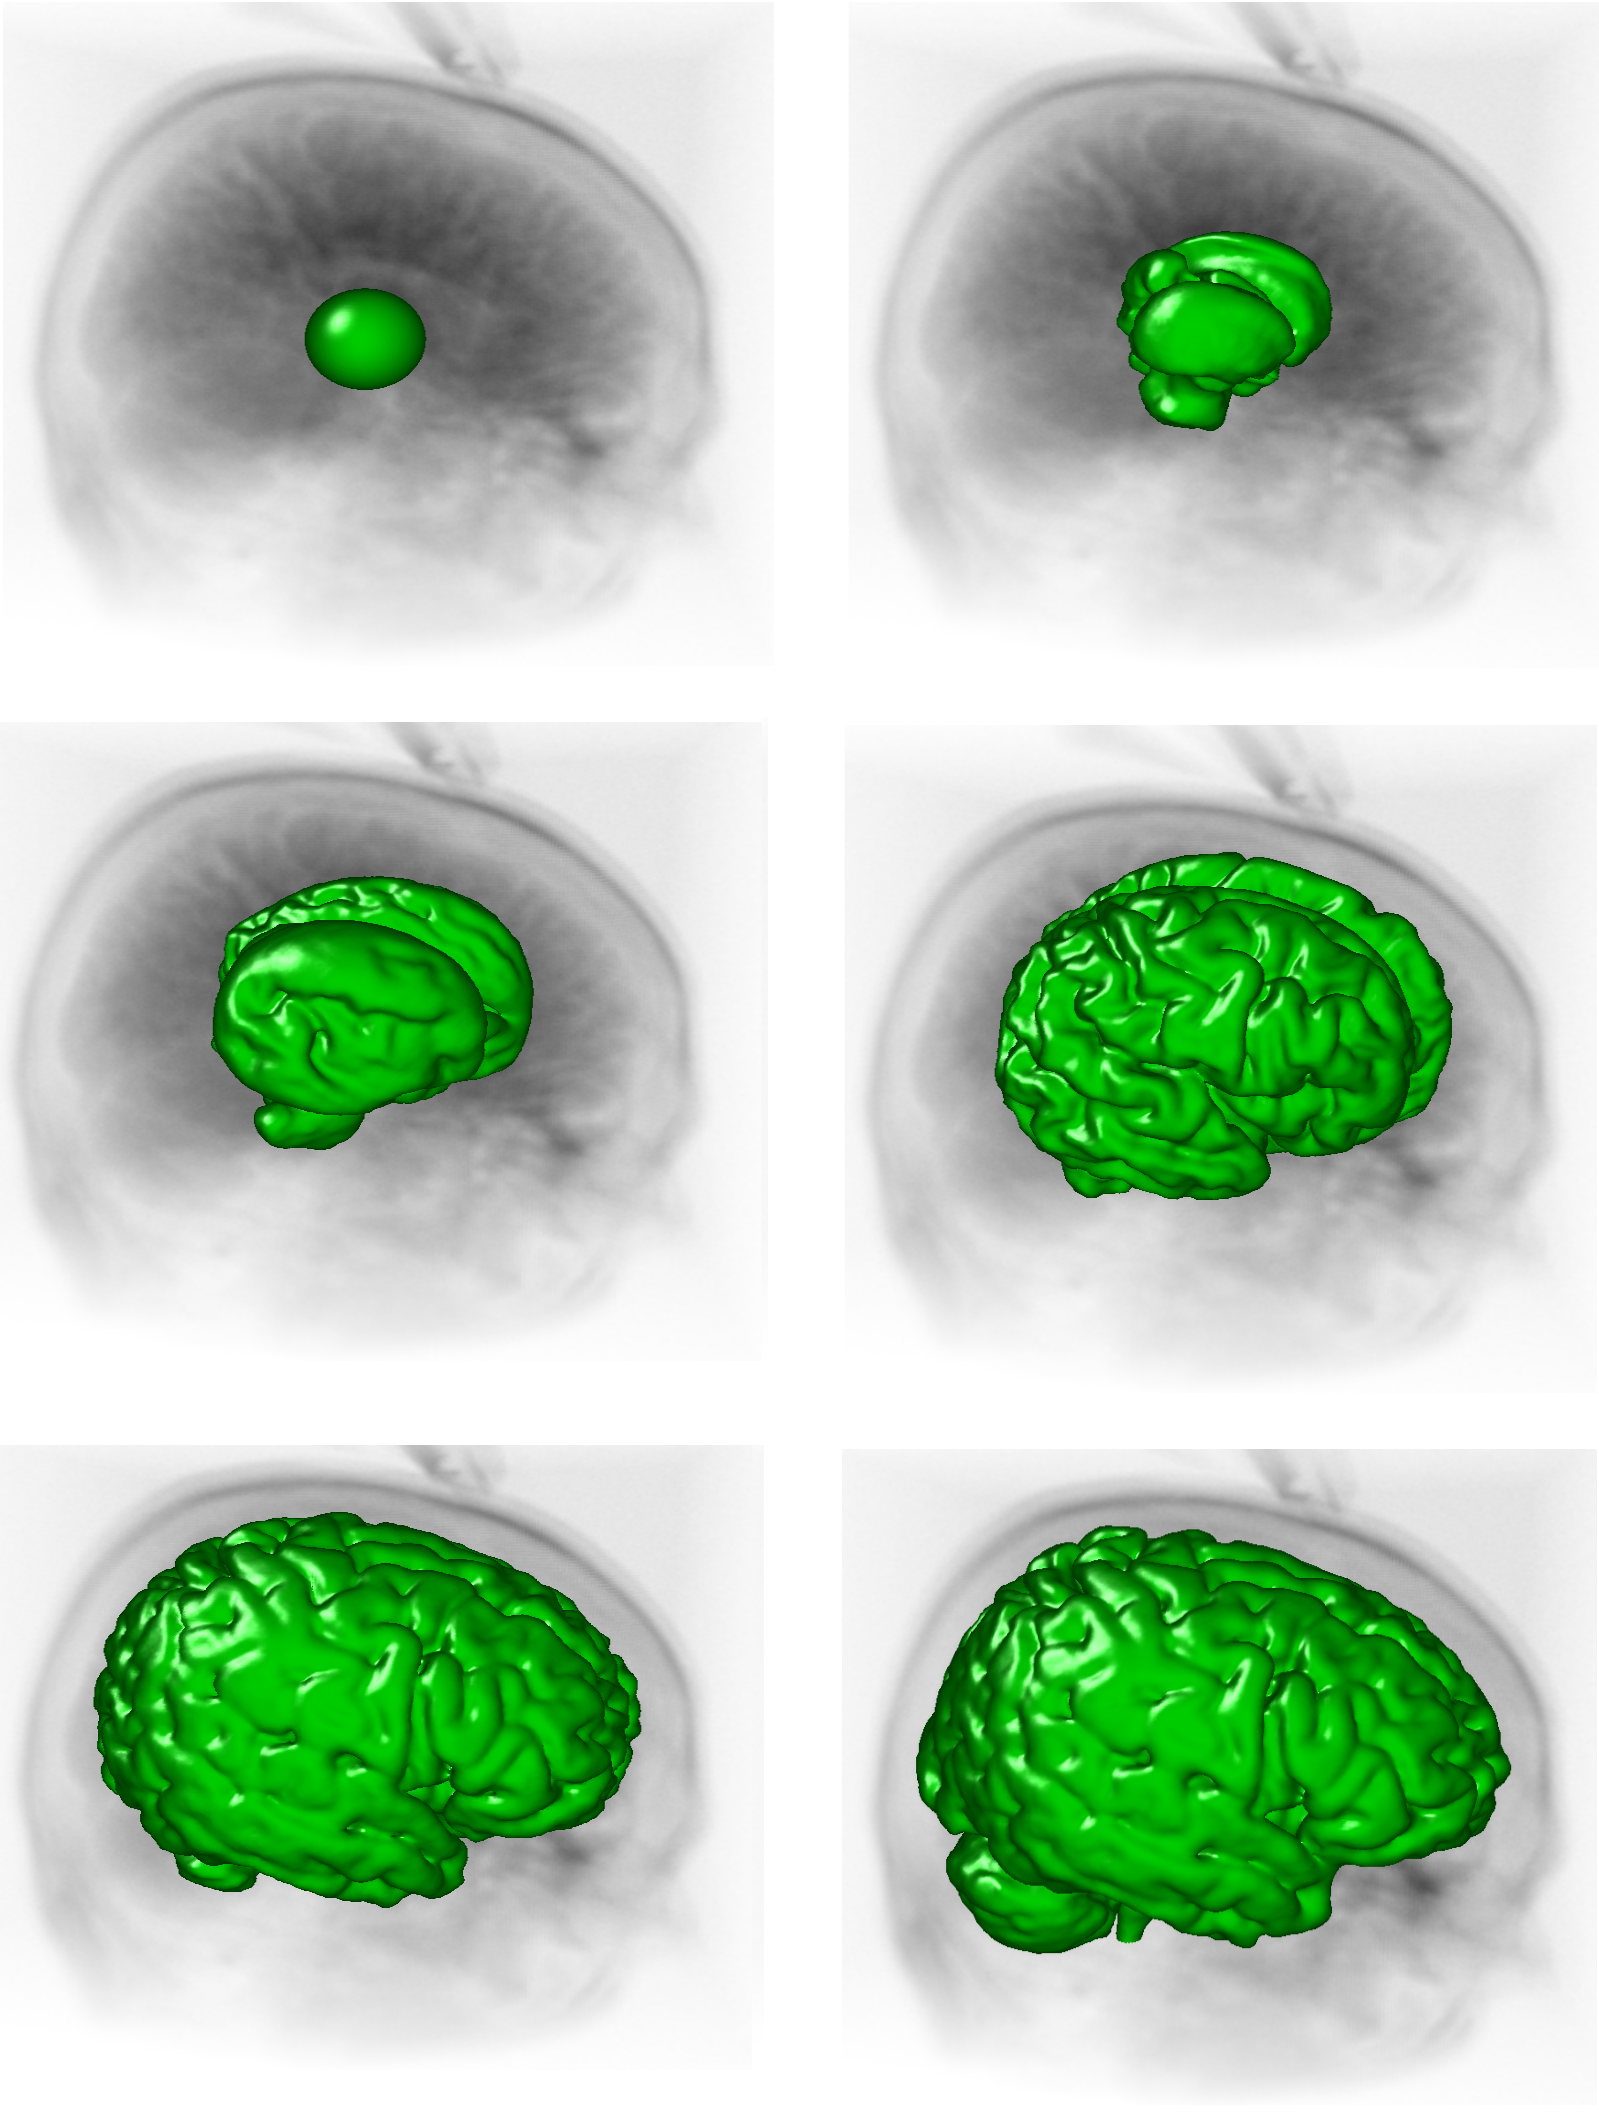
\includegraphics[width=6.0in]{figures/Brainweb-3D-Composite-NoText.png}
\caption{The progression of my algorithm while segmenting the white and grey matter in a $256^3$ head MRI with a signal-to-noise ratio of 11. The total computation time required to produce this segmentation was 7 seconds.}
\label{fig:brainweb3d}
\end{figure}
%*******************************************************************************

%*******************************************************************************
% FIGURE BrainWeb 2D
\begin{figure}[t]
\centering
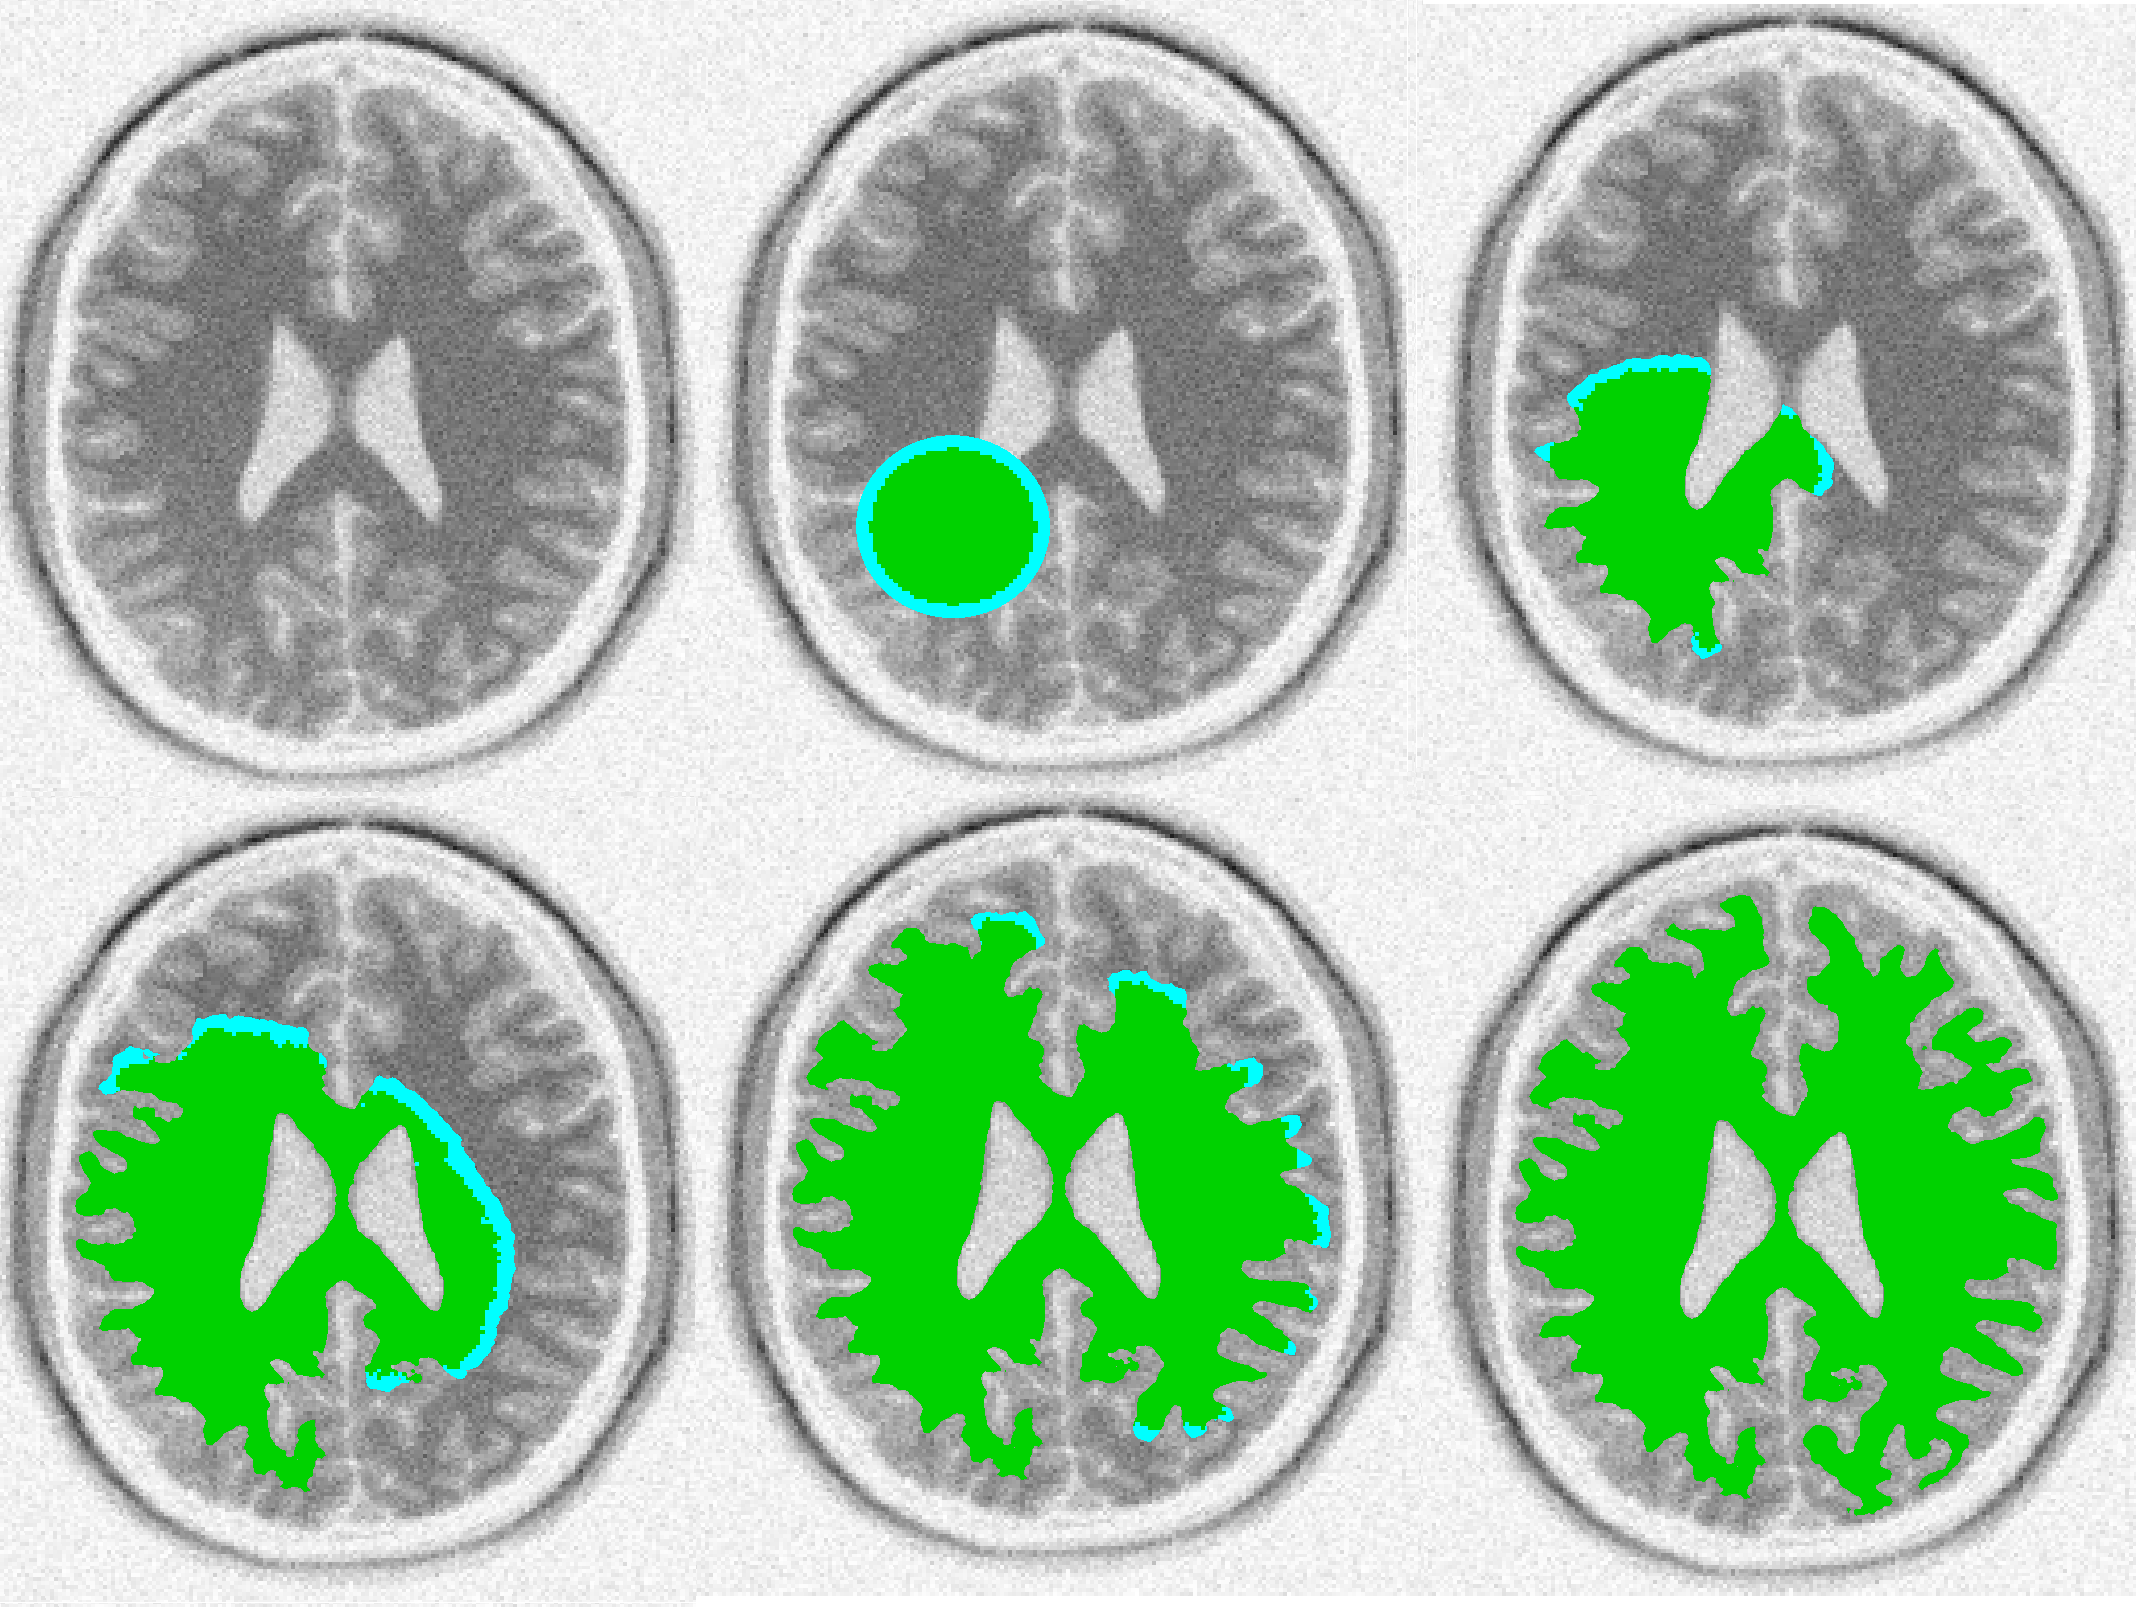
\includegraphics[width=6.0in]{figures/Brainweb-2D-Composite-2-3.png}
\caption{The progression of the active computational domain (shown in blue) with my algorithm while segmenting the white matter in a $256^3$ head MRI. Regions that have locally converged are immediately marked as inactive due to my analysis of the temporal and spatial derivatives of the level set field. The size of the active computational domain drops to zero when the segmentation has globally converged.}
\label{fig:brainweb2d}
\end{figure}
%*******************************************************************************
%*******************************************************************************
% FIGURE Accuracy
\begin{figure}[t]
\centering
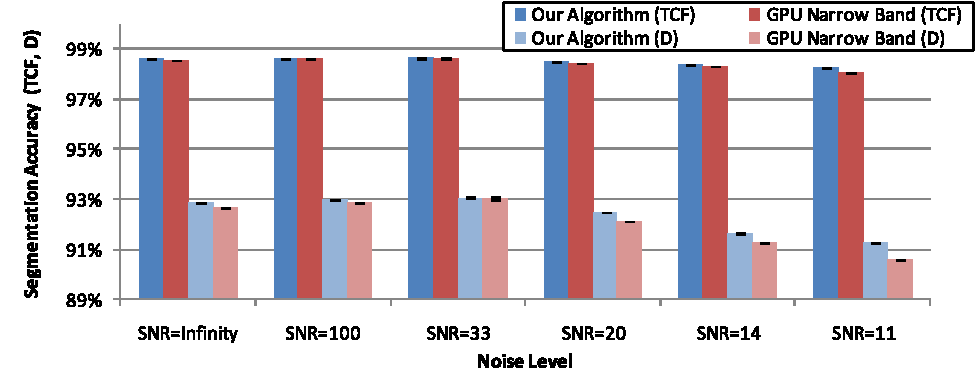
\includegraphics[width=6.0in]{figures/Accuracy.pdf}
\caption{Accuracy of my algorithm and the GPU narrow band algorithm while performing a set of repeated (N=10) white matter segmentations in a $256^3$ head MRI with varying signal-to-noise-ratio (SNR) values. For each segmentation I used a randomly selected seed point and I measured the Dice Coefficient (D) and Total Correct Fraction (TCF).}
\label{fig:8}
\end{figure}
%*******************************************************************************

%*******************************************************************************
% FIGURE Active Computational Domain per Iteration
\begin{figure}[t]
\centering
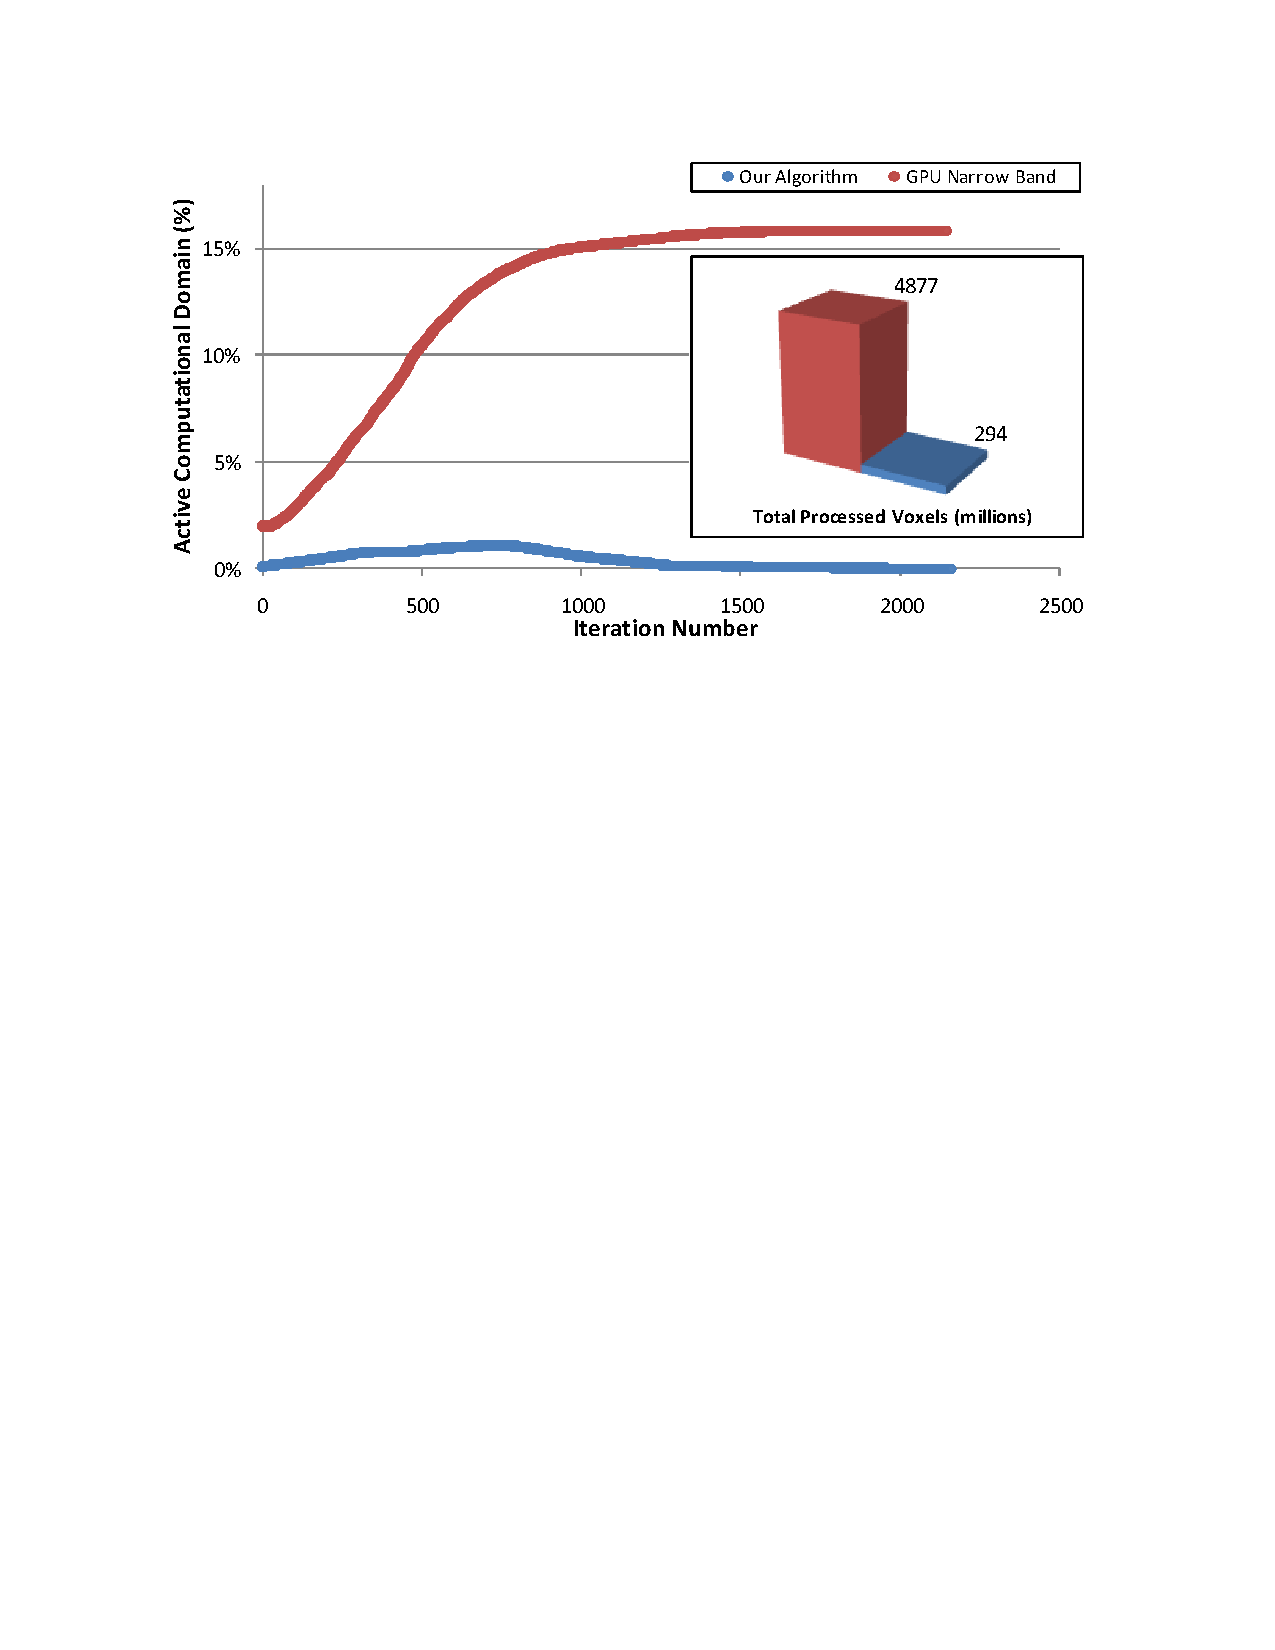
\includegraphics[width=6.0in]{figures/SpeedA1.pdf}
\caption{Size of the active computational domain per iteration for my algorithm and the GPU narrow band algorithm while segmenting the white and grey matter in a $256^3$ head MRI. The total number of grid elements processed by each algorithm is the definite integral of that algorithm's curve on this plot. These integrals are shown in the inset. Lower is better.}
\label{fig:activecomp}
\end{figure}
%*******************************************************************************

%*******************************************************************************
% FIGURE Speed per Iteration
\begin{figure}[t]
\centering
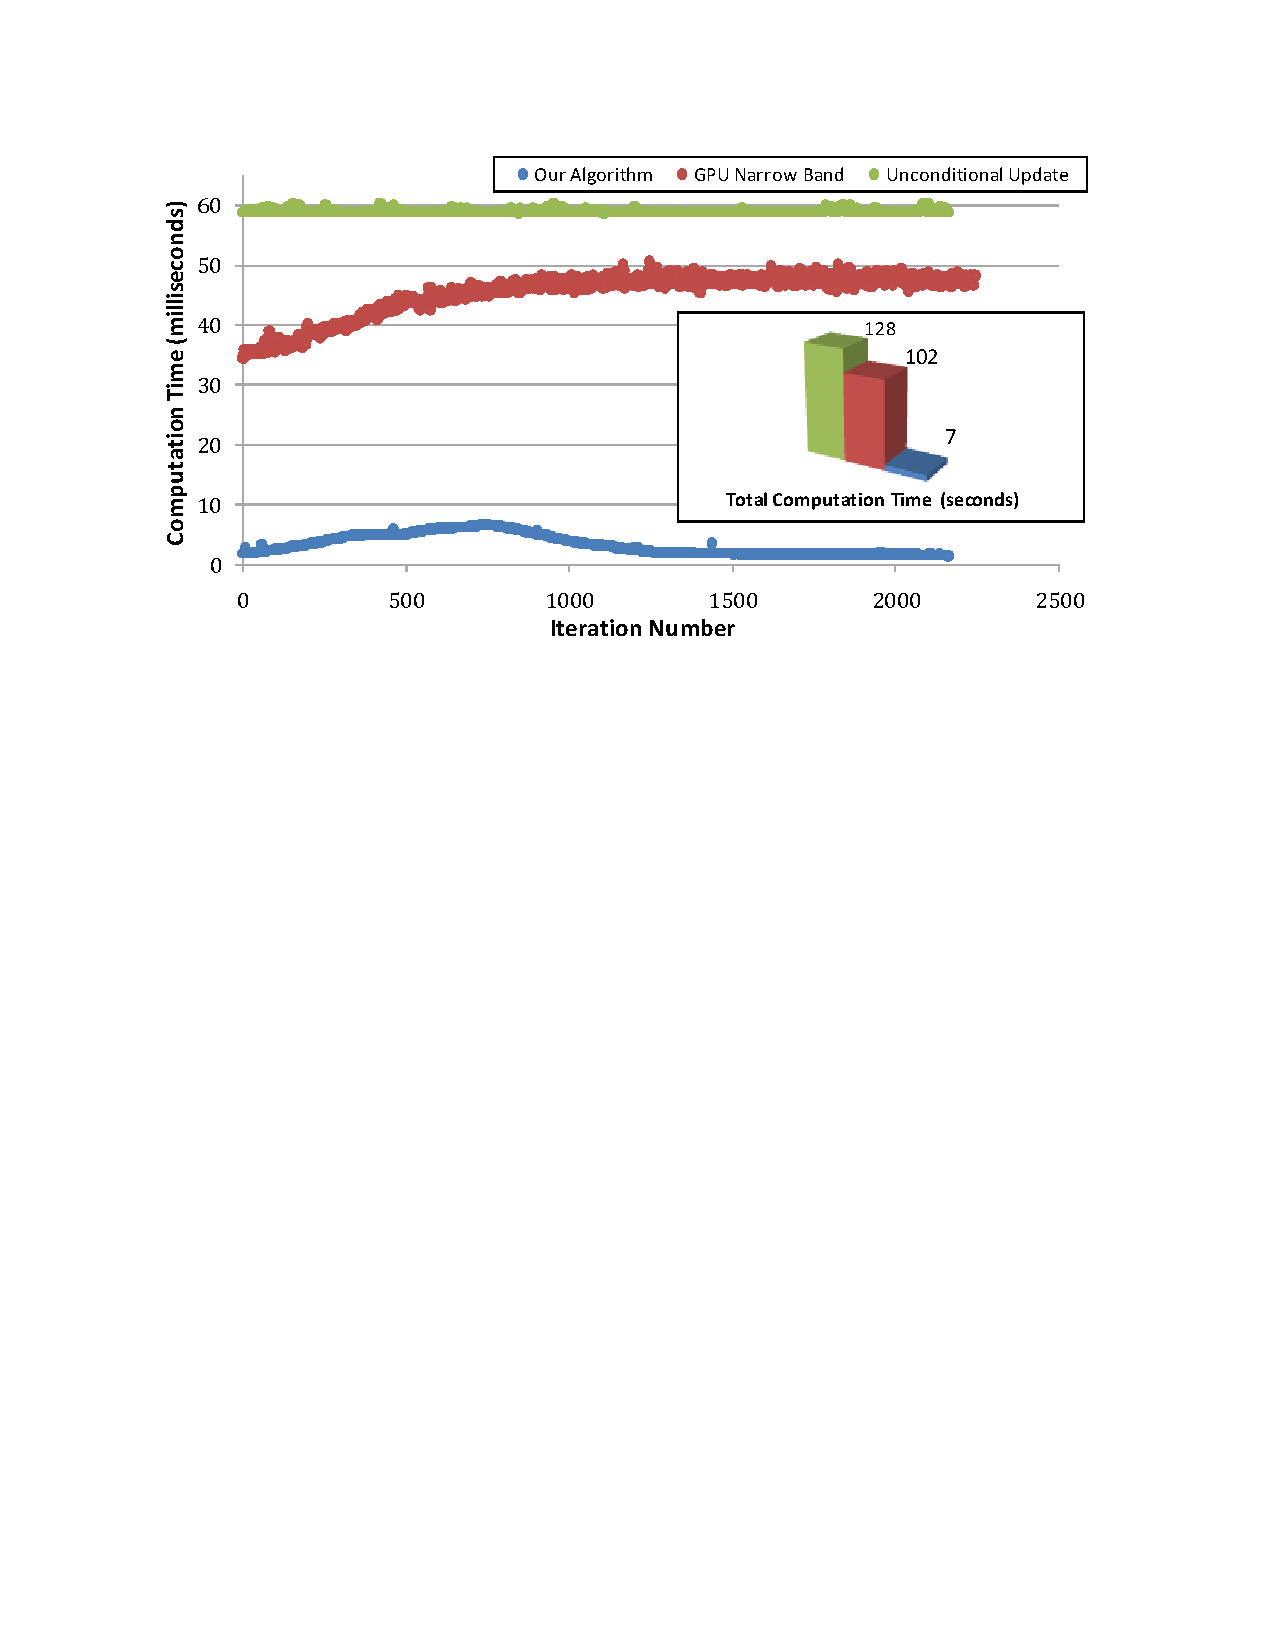
\includegraphics[width=6.0in]{figures/SpeedB1.pdf}
\caption{Computation time per iteration for my algorithm and the GPU narrow band algorithm while segmenting the white and grey matter in a $256^3$ head MRI. The total computation time for each algorithm is the integral of that algorithm's curve on this plot. These integrals are shown in the inset. Lower is better.}
\label{fig:speed}
\end{figure}
%*******************************************************************************

%*******************************************************************************
% FIGURE Speed per Active Computational Domain
\begin{figure}[t]
\centering
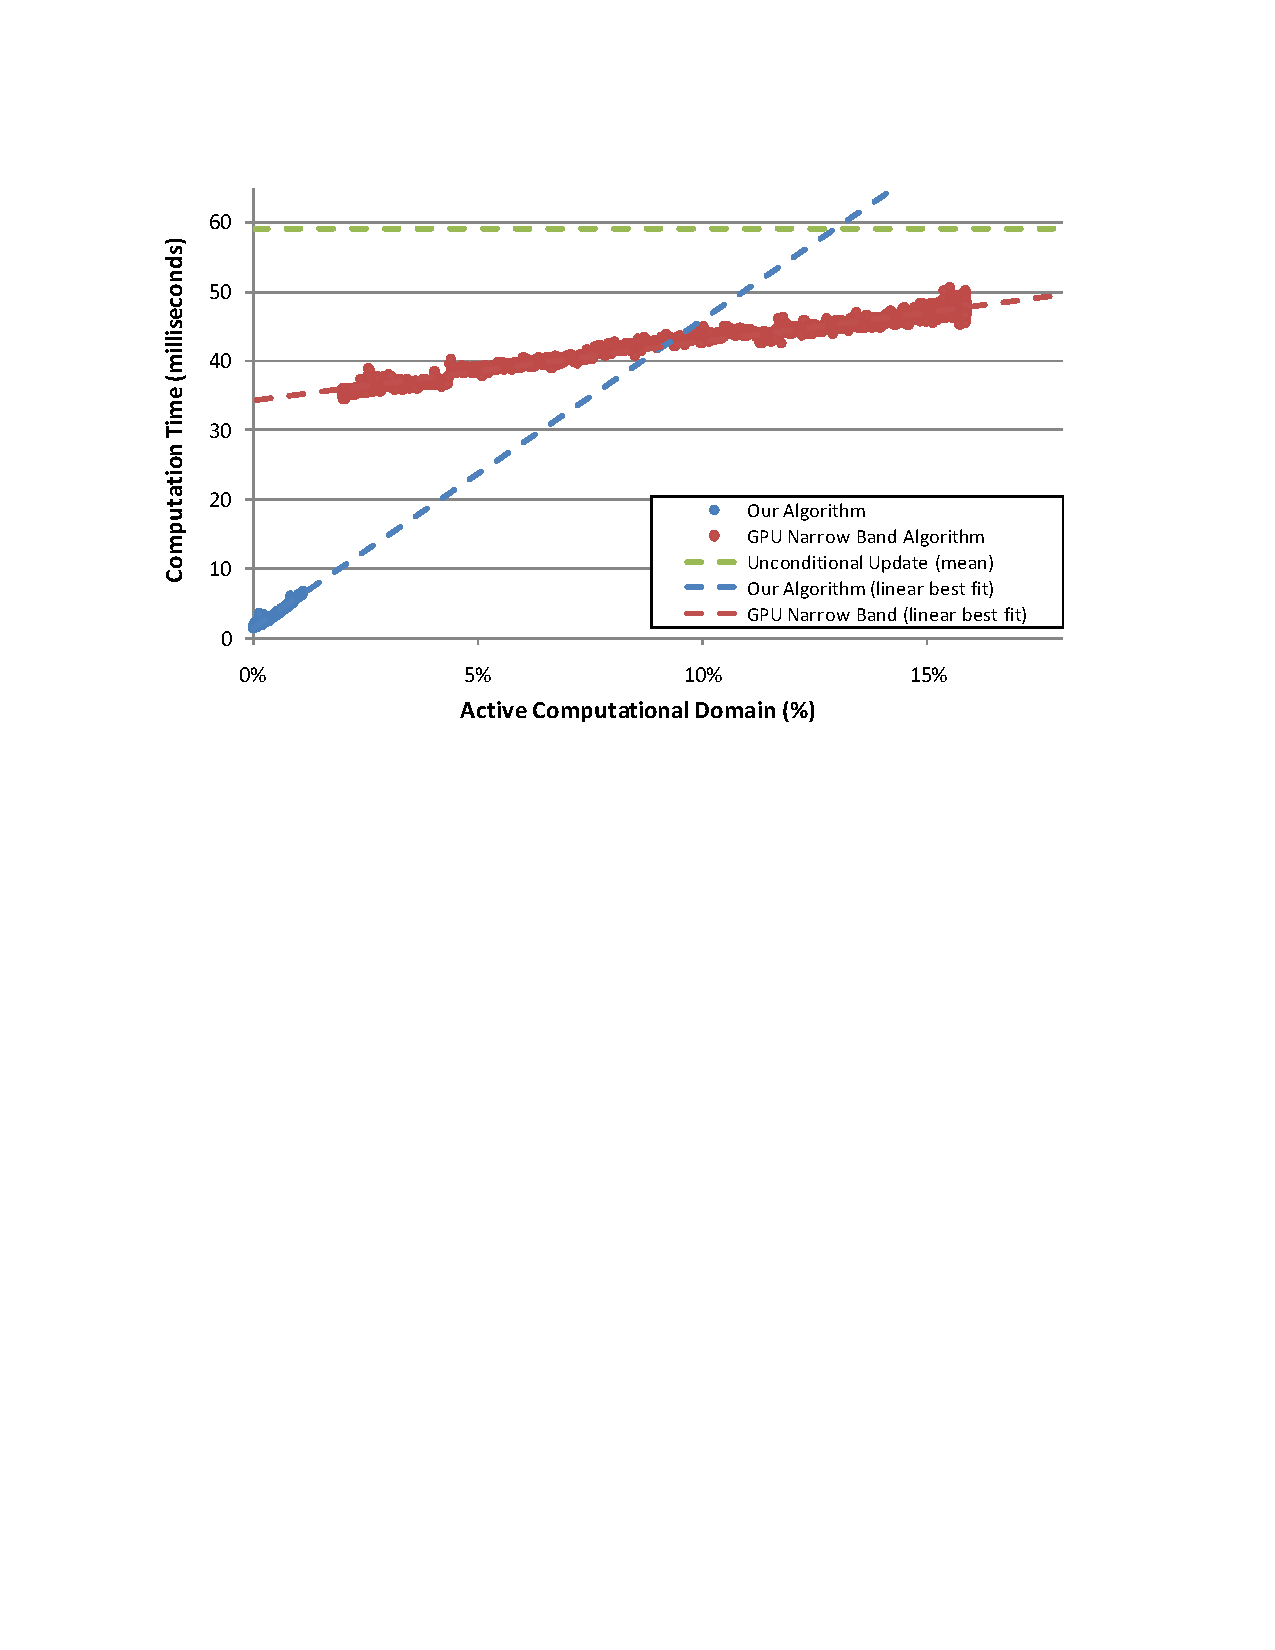
\includegraphics[width=6.0in]{figures/SpeedC1.pdf}
\caption{Computation time as a function of active computational domain size for my algorithm and the GPU narrow band algorithm while segmenting the white and grey matter in a $256^3$ head MRI. I overlay the lines of best fit for each algorithm. Lower is better.}
\label{fig:speedperactive}
\end{figure}
%*******************************************************************************

%*******************************************************************************
% FIGURE Speed per Subroutine
\begin{figure}[t]
\centering
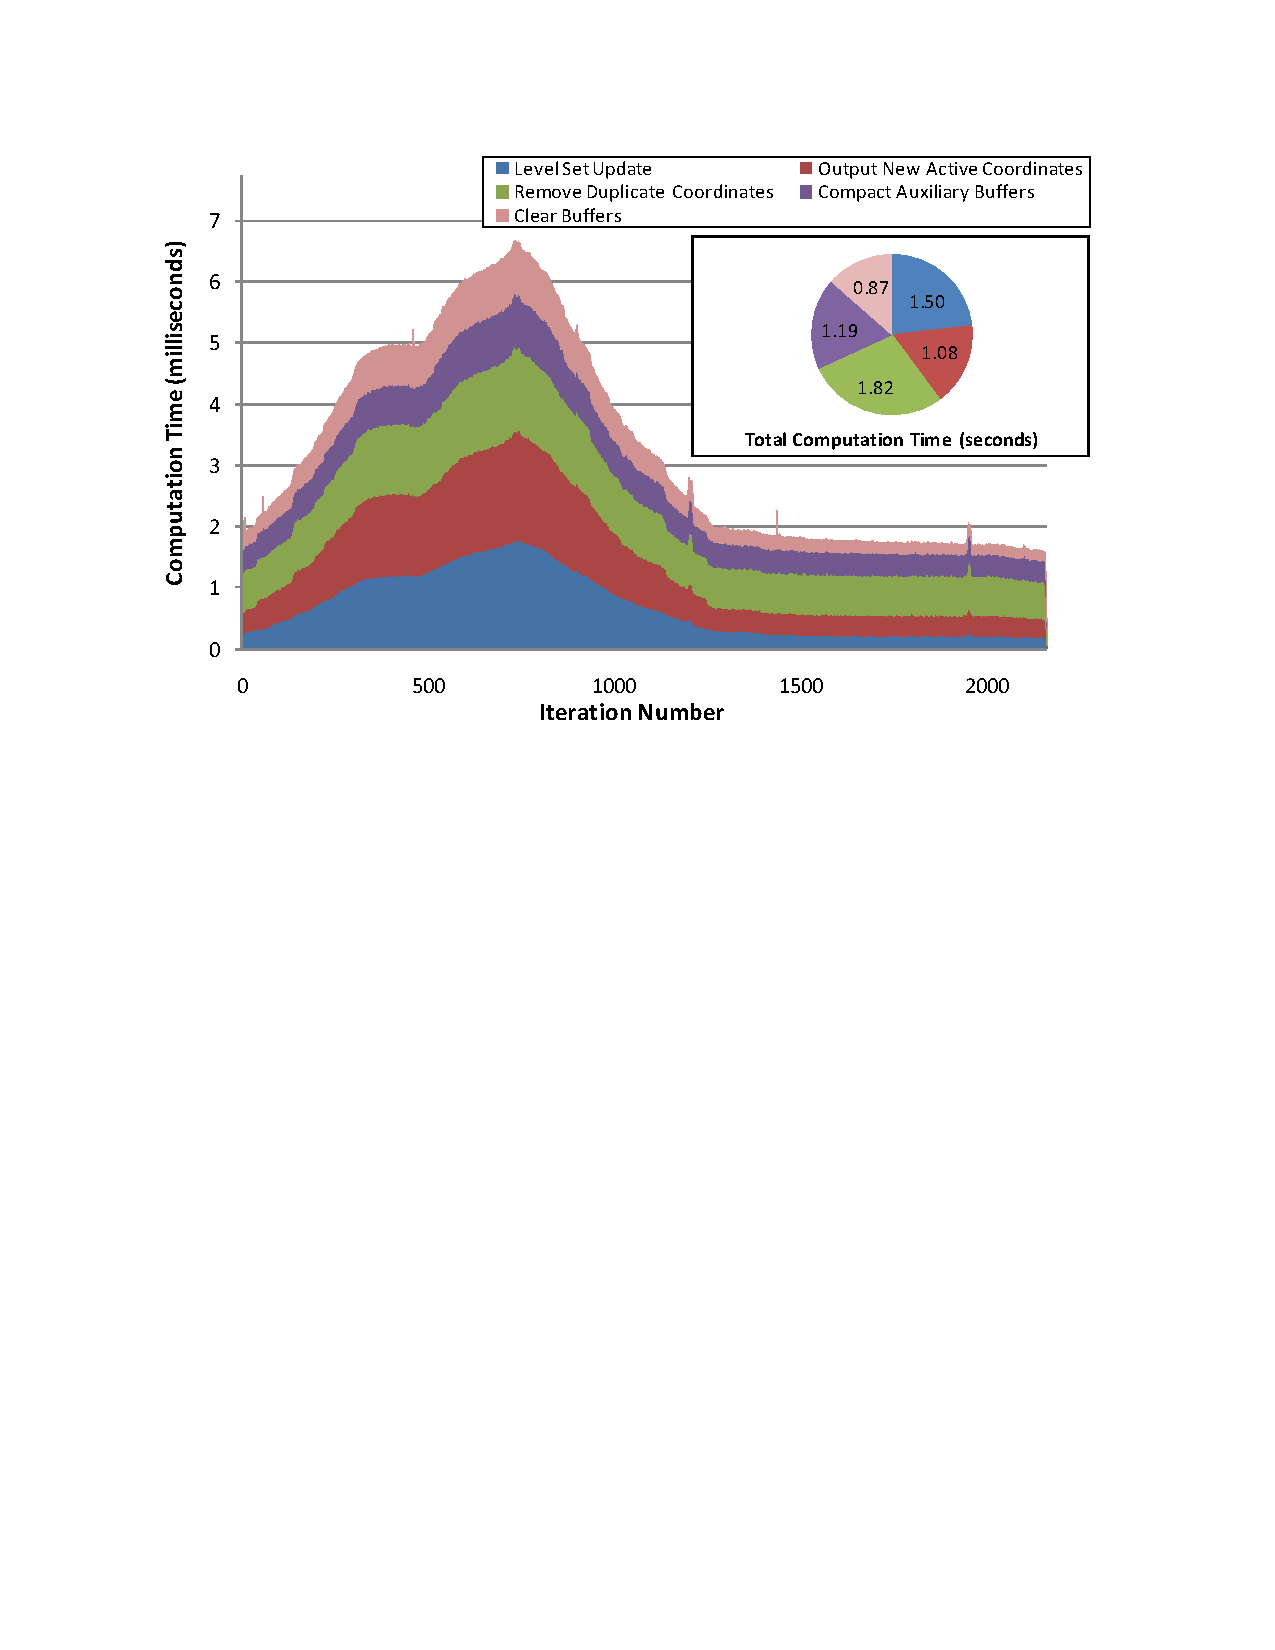
\includegraphics[width=6.0in]{figures/SpeedD1.pdf}
\caption{Computation time per iteration for each subroutine of my algorithm while segmenting the white and grey matter in a $256^3$ head MRI. Lower is better.}
\label{fig:speedpersubroutine}
\end{figure}
%*******************************************************************************

Figure~\ref{fig:aorta} and Figure~\ref{fig:bone} show qualitatively accurate segmentations produced with my algorithm. Figure~\ref{fig:brainweb3d} shows the progression of my algorithm while segmenting the white and grey matter in a ${256}^3$ head MRI with $SNR=11$. Figure~\ref{fig:brainweb2d} shows the progression of the active computational domain while segmenting the white matter in the same MRI.

I compare the accuracy of my algorithm and the GPU narrow band algorithm in Figure~\ref{fig:8}. I observed that my algorithm was slightly more accurate than the GPU narrow band algorithm with less than 0.2\% variability in all experiments. I speculate that this slight accuracy improvement is due to different floating point precision semantics in CUDA and GLSL. The accuracies I observed are comparable to those reported by Lefohn et al.~\cite{Lefohn-2003-MICCAI} and Cates et al.~\cite{Cates-2004}.

I compare the performance of my algorithm and the GPU narrow band algorithm in Figure~\ref{fig:activecomp} and Figure~\ref{fig:speed}. I observed that with my algorithm, the number of active voxels quickly peaked and decreased over time due to my analysis of the temporal and spatial derivatives of the level set field. With the GPU narrow band algorithm, the number of active voxels monotonically increased over time (Figure~\ref{fig:activecomp}). I observed that after the number of active voxels had peaked, the speed of my algorithm increased over time in contrast to the GPU narrow band algorithm (Figure~\ref{fig:speed}).

I observed that segmenting the white and grey matter in a ${256}^3$ T1w MRI with $SNR=11$ using the Insight Segmentation and Registration Toolkit took 81 minutes and 4 seconds.

Based on the observed linear relationships between the number of active voxels per iteration and the computation time per iteration (Figure~\ref{fig:speedperactive}), I conclude that the computational domain would need to be roughly 12\% active before unconditionally updating every voxel would provide a performance benefit over my algorithm. At first glance it may seem as though the GPU narrow band algorithm would provide a performance benefit over my algorithm after the computational domain is roughly 9\% active. However due to the GPU narrow band algorithm processing data in 2D tiles of size $g^2$, an active computational domain of size $n$ using my algorithm will result in a larger active computational domain of size $q$ where $n\le q\le g^2n$ using the GPU narrow band algorithm. I observed that the computational domain remained less than 2\% active during each iteration of my algorithm in all experiments.


I observed that tracking the active computational domain using my algorithm accounted for 77\% of the total computation time and updating the level set field accounted for the remaining 23\% of the total computation time (Figure~\ref{fig:speedpersubroutine}). I conclude that although most of my computation time goes into tracking the active computational domain, I leverage this cost to avoid the bigger downstream cost of unconditionally updating the entire level set field.


\include{60-results}
\fancyhead[RO,LE]{\thepage}
\fancyfoot{} 
\chapter{Conclusions}
\label{chapter:conclusions}

\section{Summary}

I have presented a new GPU level set segmentation algorithm with immediate applications in computer vision and medical imaging. My algorithm is the first and only GPU level set segmentation algorithm to be presented in the literature with linear work-complexity and logarithmic step-complexity. Moreover my algorithm makes use of a novel condition on the temporal derivatives of the level set field to limit the active computational domain to the minimal set of changing grid elements. These innovations improve computational efficiency without affecting segmentation accuracy and create new possibilities for clinical application where speed and interactivity are critical.

\section{Future Work}

The results in this thesis lead to many interesting open research questions. Since Jeong et al.\ developed their GPU narrow band algorithm concurrently to the work in this thesis, I do not empirically compare the performance of my algorithm against theirs. I only offer a theoretical argument for why my algorithm is more efficient. It would be interesting to investigate the performance of both algorithms in a controlled fashion to discover how the theoretical step-complexity of each algorithm translates into practical performance.

The parallel algorithm presented in this thesis is clearly limited by the amount of memory it requires. An interesting avenue for future research would be to investigate how maintain and traverse a sparse representation of the level set field in parallel. In this sense, the level set solver I propose would be sparse in both the computational and storage domains. There has been some interesting recent work on efficiently maintaining such a sparse representation sequentially on the CPU~\cite{Houston-2006,Nielsen-2006,Nielsen-2007}, however this work explicitly states that efficient access to the level set field is guaranteed only when it is accessed sequentially.

Another interesting avenue for future research would be to extend the optimizations presented in this thesis to speed functions that look at larger local neighborhoods. The memory requirements of the algorithm presented in this thesis scale linearly with the number of neighbors examined by each thread in the level set solver. Depending on the number of neighbors examined by the speed
function, different strategies for maintaining the active domain and maximizing cache locality may offer superior performance over the algorithm described in this thesis.

Investigating how a user could intuitively paint on the medical data to communicate intent and domain expertise to the level set solver in real time is another interesting avenue for future research.

Finally it would be interesting to extend the optimized level set algorithm described in this thesis beyond the field of medical imaging into the many problem domains already leveraging level set formulations, such as surface reconstruction and fluid simulation.  

% In future we plan to perform a detailed bottleneck analysis to learn more about the relationships between computation and communication inherent in our algorithm and the GPU narrow band algorithm. We also plan to investigate strategies for further improving the cache coherence of our sparse active computational domain. Finally we plan to investigate how our algorithm can be extended to higher-order space and time discretization schemes involving bigger local neighborhoods.



\phantomsection

\bibliographystyle{plain}
\bibliography{bibliography}

\appendix

\phantomsection
\fancyhead[RO,LE]{\thepage}
\fancyfoot{} 
\chapter{Derivation of the Active Set Membership Condition $ \varsigma_{2} $ }
\label{app:temporal}

I define the set of all user-specified parameters to the speed function as $H$ and the user-specified image as $I$. I define $\eta \left({\mathbf x}\right)=\{{\mathbf x},{{\mathbf n}}^{{\mathbf x}}_0,{{\mathbf n}}^{{\mathbf x}}_1,{{\mathbf n}}^{{\mathbf x}}_2,\ldots ,{{\mathbf n}}^{{\mathbf x}}_k\}$ to be the set of coordinates in the immediate neighborhood of some voxel ${\mathbf x}$. I define the set of all of level set field values in the immediate neighborhood of ${\mathbf x}$ at time $t$ as follows:
%*******************************************************************************
\begin{equation}
\Phi \left({\mathbf x},t\right)=\{\phi\left({\mathbf x},t\right),\phi\left({{\mathbf n}}^{{\mathbf x}}_0,t\right),\phi\left({{\mathbf n}}^{{\mathbf x}}_1,t\right),{\phi({\mathbf n}}^{{\mathbf x}}_2,t),\ldots ,{\phi({\mathbf n}}^{{\mathbf x}}_k,t)\}
\end{equation}
%*******************************************************************************
I assume that the speed function $F({\mathbf x},t)$ is a function of the level set values around ${\mathbf x}$ during the previous iteration $\Phi \left({\mathbf x},t-\Delta t\right)$, the image $I$, and the set of user-specified parameters $H$. I assume without loss of generality that $\Delta t\ne 0$.

I want to prove that ${\forall }_{{\mathbf n}\in \eta \left({\mathbf x}\right)}:\phi\left({\mathbf n},t-\Delta t\right)=\phi({\mathbf n},t-2\Delta t)$ implies $\phi\left({\mathbf x},t\right)=\phi\left({\mathbf x},t-\Delta t\right)$. If this claim is true, it means that I can exclude $\mathbf{x}$ from the active set at time $t$ if ${\forall }_{{\mathbf n}\in \eta \left({\mathbf x}\right)}:\phi\left({\mathbf n},t-\Delta t\right)=\phi({\mathbf n},t-2\Delta t)$. I begin by proving a useful lemma.

\medskip

\medskip

\medskip

\medskip

\begin{quote}
\textbf{Lemma} \ \
$\Phi \left({\mathbf x},t-\Delta t\right)=\Phi \left({\mathbf x},t-2\Delta t\right)$ implies $F\left({\mathbf x},t\right)=F\left({\mathbf x},t-\Delta t\right)$.

\textbf{Proof} \ \ \ \ \ I assume $\Phi \left({\mathbf x},t-\Delta t\right)=\Phi \left({\mathbf x},t-2\Delta t\right)$. By definition,
%*******************************************************************************
\begin{equation}
F\left({\mathbf x},t\right)=f(\Phi \left({\mathbf x},t-\Delta t\right),I,H) \mbox{ for some function } f.
\end{equation}
%*******************************************************************************
Therefore I get,
%*******************************************************************************
\begin{equation}
F\left({\mathbf x},t-\Delta t\right)=f\left(\Phi \left({\mathbf x},t-2\Delta t\right),I,H\right)=f\left(\Phi \left({\mathbf x},t-\Delta t\right),I,H\right)=F\left({\mathbf x},t\right)
\end{equation}
%*******************************************************************************
\qed
\end{quote}

\medskip

\medskip

\medskip

\medskip

Now I move onto my central proof.

\medskip

\medskip

\medskip

\medskip

\begin{quote}
\textbf{Claim} \ \ \ \ 
${\forall }_{{\mathbf n}\in \eta \left({\mathbf x}\right)}:\phi\left({\mathbf n},t-\Delta t\right)=\phi({\mathbf n},t-2\Delta t)$ implies $\phi\left({\mathbf x},t\right)=\phi\left({\mathbf x},t-\Delta t\right)$.

\textbf{Proof} \ \ \ \ \
I prove by contradiction. I assume,
%*******************************************************************************
\begin{equation}
{\forall }_{{\mathbf n}\in \eta \left({\mathbf x}\right)}:\phi\left({\mathbf n},t-\Delta t\right)=\phi({\mathbf n},t-2\Delta t)
\end{equation}
%*******************************************************************************
From this expression and the definition of $\Phi$, I get,
%*******************************************************************************
\begin{equation}
\Phi \left({\mathbf x},t-\Delta t\right)=\Phi \left({\mathbf x},t-2\Delta t\right)
\end{equation}
%*******************************************************************************
From the lemma~above I get $F\left({\mathbf x},t\right)=F\left({\mathbf x},t-\Delta t\right)$. From the definition of $\nabla \phi$, I get $\nabla \phi\left({\mathbf x},t - \Delta t\right) = \nabla \phi\left({\mathbf x},t - 2 \Delta t\right)$.

\medskip

\medskip

\medskip

\medskip

I assume for the sake of contradiction that $\phi\left({\mathbf x},t\right)\ne \phi\left({\mathbf x},t-\Delta t\right)$. Substituting this inequality into Equation~\ref{eq:levelseteq} I get,
%*******************************************************************************
\begin{equation}
\phi\left({\mathbf x},t\right)-\phi\left({\mathbf x},t-\Delta t\right)=\Delta tF\left({\mathbf x},t\right)\left|\nabla \phi\left({\mathbf x},t-\Delta t\right)\right|\ne 0
\end{equation}
%*******************************************************************************

From the zero product rule I get $F\left({\mathbf x},t\right)\ne 0$ and $\left|\nabla \phi\left({\mathbf x},t-\Delta t\right)\right|\ne 0$.

\medskip

\medskip

\medskip

\medskip

From my initial assumption that ${\forall }_{{\mathbf n}\in \eta \left({\mathbf x}\right)}:\phi\left({\mathbf n},t-\Delta t\right)=\phi({\mathbf n},t-2\Delta t)$, and since ${\mathbf x}\in \eta \left({\mathbf x}\right)$, I get $\phi\left({\mathbf x},t-\Delta t\right)=\phi({\mathbf x},t-2\Delta t)$. Substituting the right hand side of this expression into Equation~\ref{eq:levelseteq} I get,
%*******************************************************************************
\begin{equation}
\phi\left({\mathbf x},t-\Delta t\right)=\phi\left({\mathbf x},t-\Delta t\right)+\Delta tF\left({\mathbf x},t-\Delta t\right)\left|\nabla \phi\left({\mathbf x},t-2\Delta t\right)\right|
\end{equation}
%*******************************************************************************
or equivalently,
%*******************************************************************************
\begin{equation}
\Delta tF\left({\mathbf x},t-\Delta t\right)\left|\nabla \phi\left({\mathbf x},t-2\Delta t\right)\right|=0
\end{equation}
%*******************************************************************************
From this expression and the zero product rule I get either $F\left({\mathbf x},t-\Delta t\right)=0$ or $\left|\nabla \phi\left({\mathbf x},t-2\Delta t\right)\right|=0$.

\medskip

\medskip

\medskip

\medskip

I assume for the moment that $F\left({\mathbf x},t-\Delta t\right)=0$. Since $F\left({\mathbf x},t\right)=F\left({\mathbf x},t-\Delta t\right)$ I get $F\left({\mathbf x},t\right)=0$ which leads to a contradiction. Now I assume for the moment that $\left|\nabla \phi\left({\mathbf x},t-2\Delta t\right)\right|=0$. From this expression, and since $\nabla \phi\left({\mathbf x},t - \Delta t\right) = \nabla \phi\left({\mathbf x},t - 2 \Delta t\right)$, I get $\left|\nabla \phi\left({\mathbf x},t-\Delta t\right)\right|=0$ which also leads to a contradiction. Therefore $\phi\left({\mathbf x},t\right)=\phi\left({\mathbf x},t-\Delta t\right)$. \qed

\end{quote}


\phantomsection
\fancyhead[RO,LE]{\thepage}
\fancyfoot{} 
\chapter{Proof That My Algorithm is Work-Efficient and Step-Efficient}
\label{app:proof}

I prove that my parallel algorithm is both work-efficient and step-efficient by considering each of its subroutines individually. I define $n$ as the size of the active computational domain and $p$ as the size of the entire level set field.
Listing~\ref{pseudo:1} requires one pass over the entire computational domain and therefore has $O(p)$ work-complexity and $O(1)$ step-complexity.

The \textbf{for all} loop in Listing~\ref{pseudo:2} requires one pass over the entire computational domain and therefore has $O(p)$ work-complexity and $O(1)$ step-complexity. The call to \textbf{compact} in Listing~\ref{pseudo:2} has $O(p)$ work-complexity and $O({\log}_2 p)$ step-complexity~\cite{Harris-2007,Sengupta-2007,Sengupta-2011}.

Listing~\ref{pseudo:3} and Listing~\ref{pseudo:4} each require one pass over the active computational domain and therefore each has $O(n)$ work-complexity and $O(1)$ step-complexity.

Listing~\ref{pseudo:5} requires seven passes over the active computational domain, not including the call to \textbf{compact}, and therefore has $O(n)$ work-complexity and $O(1)$ step-complexity. The call to \textbf{compact} in Listing~\ref{pseudo:5} has $O(n)$ work-complexity and $O({\log}_2 n)$ step-complexity~\cite{Harris-2007,Sengupta-2007,Sengupta-2011}. After Listing~\ref{pseudo:5}, my algorithm must clear $B^{\mathbf{e}}_{0 \ldots n}$ for all offset vectors $\mathbf{e} \in E$. Clearing these buffers has $O(n)$ work-complexity and $O(1)$ step-complexity.

I conclude that my algorithm has $O(p)$ work-complexity and $O({\log}_2 p)$ step-complexity during initialization. After initialization my algorithm has $O(n)$ work-complexity and $O({\log}_2 n)$ step-complexity. \qed


\phantomsection
\fancyhead[RO,LE]{\thepage}
\fancyfoot{} 
\chapter{Publications}
\label{app:publications}

The research in this thesis makes the following contributions.

\section{Refereed Conference Papers}

\begin{noindent}Mike Roberts, Jeff Packer, Mario Costa Sousa, Joseph Ross Mitchell. A work-efficient GPU algorithm for level set segmentation. In \emph{ACM SIGGRAPH/Eurographics Conference on High Performance Graphics 2010 (HPG '10)}. pages 123--132, June 2010.\end{noindent}

\section{Refereed Oral Presentations}

\begin{noindent}Mike Roberts, Jeff Packer, Mario Costa Sousa, Joseph Ross Mitchell. A work-efficient GPU algorithm for level set segmentation. Oral presentation at \emph{Nvidia GPU Technology Conference Research Summit 2010 (GTC '10)}. September 2010.\end{noindent}

\bigskip

\begin{noindent}Mike Roberts, Eric Penner, Jeff Packer, Mario Costa Sousa, Joseph Ross Mitchell. Advanced medical volume rendering and segmentation on the GPU. Oral presentation at \emph{Nvidia GPU Technology Conference Research Summit 2010 (GTC '10)}. September 2010.\end{noindent}

\bigskip

\begin{noindent}Mike Roberts, Jeff Packer, Mario Costa Sousa, Joseph Ross Mitchell. Level set segmentation of large medical data sets on modern graphics hardware. In \emph{10th Annual Alberta Biomedical Engineering Conference 2009}. page 24. October 2009.\end{noindent}

\section{Refereed Posters}

\begin{noindent}Mike Roberts, Jeff Packer, Mario Costa Sousa, Joseph Ross Mitchell. Interactive 3D level set segmentation on modern graphics hardware. Oral presentation at \emph{Radiological Society of North America Annual Meeting 2010 (RSNA '10)}. November 2010.\end{noindent}

\bigskip

\begin{noindent}Mike Roberts, Mario Costa Sousa, Joseph Ross Mitchell. A work-efficient GPU algorithm for level set segmentation. Poster at \emph{ACM SIGGRAPH 2010}. July 2010. \textbf{ACM SIGGRAPH Student Research Competition Semi-Finalist}.\end{noindent}

\bigskip

\begin{noindent}Mike Roberts, Jeff Packer, Mario Costa Sousa, Joseph Ross Mitchell. Using desktop graphics processors in diagnostic medicine. Poster at \emph{University of Calgary Graduate Conference 2010}. May 2010. \textbf{Natural Sciences and Engineering Research Council of Canada (NSERC) Best Poster Award}.\end{noindent}

\bigskip

\begin{noindent}Mike Roberts, Jeff Packer, Mario Costa Sousa, J. Ross Mitchell. Level set segmentation of large medical data sets on modern graphics hardware. Poster at \emph{25th Anniversary Alberta Cancer Research Institute Research Meeting 2009}. November 2009.\end{noindent}

\bigskip

\begin{noindent}Mike Roberts, Jeff Packer, J. Ross Mitchell, Mario Costa Sousa. CUDA-accelerated sparse-field level set segmentation of large medical data sets on modern graphics hardware. Poster at \emph{Nvidia GPU Technology Conference Research Summit 2009 (GTC '09)}. September 2009.\end{noindent}

\section{Patents}

\begin{noindent}Mike Roberts, Joseph Ross Mitchell, Mario Costa Sousa. Parallel process for level set segmentation of volume data. \emph{United States Patent filed on June 7th, 2010}.\end{noindent}

\bigskip

\begin{noindent}Mike Roberts, Joseph Ross Mitchell, Mario Costa Sousa. Level set segmentation of volume data. \emph{United States Provisional Patent filed on September 25th, 2009}.\end{noindent}


\phantomsection
\fancyhead[RO,LE]{\thepage}
\fancyfoot{} 
\chapter{A Work-Efficient GPU Algorithm for Level Set Segmentation}
\label{app:hpg}

Mike Roberts, Jeff Packer, Mario Costa Sousa, Joseph Ross Mitchell. A work-efficient GPU algorithm for level set segmentation. In \emph{ACM SIGGRAPH/Eurographics Conference on High Performance Graphics 2010 (HPG '10)}. pages 123--132, June 2010.



\end{document}


